\documentclass[a4paper,12pt]{ctexart}
\usepackage{../../teaching-style}
\usepackage{tikz}
\usetikzlibrary{arrows.meta,calc}
\usepackage{hyperref}
\hypersetup{colorlinks=true,linkcolor=mainblue}

\begin{document}
\pagestyle{empty}

% ===== 封面 =====
\vspace*{2.5cm}
{\centering
  {\Huge\bfseries\color{mainblue} 线性代数初步}\par
  \vspace{0.6cm}
  {\Large 从几何变换到二次型}\par
  \vspace{2cm}
  \rule{0.5\textwidth}{0.4pt}\par
  \vspace{1.2cm}
  {\normalsize 适用学段：高中一\~{}三年级（课外扩展模块）}\par
  \vspace{0.4cm}
  {\normalsize 先修要求：平面解析几何、平面向量、三角函数基础}\par
  \vspace{0.4cm}
  {\normalsize 建议课时：30\~{}36 课时（含练习）}\par
  \vspace{1.2cm}
  \rule{0.5\textwidth}{0.4pt}
}
\newpage

% ===== 使用说明 =====
\vspace*{0.5cm}
{\Large\bfseries\color{mainblue} 使用说明}\par
\vspace{0.3cm}

\textbf{适用对象。} 本教材面向已修完平面解析几何和高中三角函数入门的学生。不需要任何线性代数预备知识——一切从坐标平面上的几何直觉出发。

\textbf{教学理念。} 全书遵循"先做足够多的具体数字例子，再总结一般规律"的原则。每一节都从手算几个具体的点或矩阵开始，让学生先看到现象，再归纳公式。这与传统从定义出发的讲法相反——我们把"为什么"放在"是什么"之前。

\textbf{章节安排。} 第一章建立几何直觉（五种变换），第二章引入矩阵语言，第三章用行列式度量面积效应，第四章发掘不变方向（特征值与特征向量），第五章用齐次坐标统一平移，第六章将全部工具汇聚于圆锥曲线分类——这是全书的高潮。第七章对前六章的概念做系统推广，引入拉普拉斯展开、克拉默法则和奇异值分解，并设有全书综合练习。

\textbf{练习体系。} 大部分节后配有即时练习，每章末设有 A 组（基础巩固）和 B 组（挑战提升）。A 组侧重计算熟练度，B 组侧重概念理解与跨节综合。全书习题约 200 题，所有答案列于书末附录。习题中的数字不刻意凑整——部分题目会出现分数、根号等"不整洁"的结果，目的是让学生习惯真实计算场景。

\textbf{致教师。} 如果课时有限，前五章可各用 3--4 课时完成，第六章用 4--5 课时（务必讲透），第七章可根据学生程度选讲或作为阅读材料。每章的"本章小结"可直接用作板书提纲。建议重点讲解各章的实例部分，让学生课后独立完成 A 组练习，B 组可作为讨论题或选做。

\newpage

\pagenumbering{arabic}
\pagestyle{plain}

\preface{前言}

这本书不走抽象定义的老路。我们从最直观的事情开始——在坐标平面上
把一个点旋转一下，把一张图反射一下，把一个图形拉长或压扁。这些动作，
你用手比划一下就能想象出来。做完足够多的例子之后，你会发现它们背后
有一个共同的结构，这个结构恰好可以用一种叫做"矩阵"的数学对象来表达。
接着，矩阵的乘法和行列式就自然出现了。然后引入特征值与特征向量，再用齐次坐标处理平移，最后用这套语言来优雅地处理
圆锥曲线——椭圆、双曲线、抛物线的分类，其实就是特征值的正负号问题。

全书遵循一个原则：\textbf{先做足够多的具体数字的例子，再总结一般规律。}
每一节后面都配有练习，每一章末尾配有两组综合练习（A组打基础，
B组挑战提升），所有习题答案附在书末。

\newpage

\chaptertitle{第一章\quad 平面上的几何变换}

本书的第一章从一个最简单的问题开始：在坐标平面上，如果我们把每个点按照某种规则挪到一个新的位置，整个图形会发生什么变化？旋转一下、翻折一下、拉长一下、推挤一下——这些在日常生活中用手就能比划的"动作"，进入数学之后就变成了精确的坐标公式。本章逐一考察五种最基本的几何变换，用大量具体数字建立直觉，最后你会发现它们竟然都写成同一种形式——这将是第二章引出"矩阵"概念的伏笔。

\sectiontitle{1.1\quad 坐标——给平面上的点一个"地址"}

取一张方格纸。在纸上画两条互相垂直的直线：水平的这条叫$x$轴，竖直的这条叫$y$轴。两条线相交的那一点叫原点，记作$O$。

现在平面上任何一个点都可以用两个数来"定位"。从原点到那个点，向右（或左）走多少格给一个数，向上（或下）走多少格再给一个数。向右和向上的方向为正，向左和向下的方向为负。这两个数分别叫该点的$x$坐标和$y$坐标，记作$(x,y)$。

\begin{example}
写出以下各点的坐标：
(1) 从原点向右2格、向上5格；
(2) 从原点向左3格、向下1格；
(3) 从原点向左4格、向上0格。
\end{example}
\begin{solution}
(1) 向右为正、向上为正，所以是$(2,5)$。\\
(2) 向左为负、向下为负，所以是$(-3,-1)$。\\
(3) 向左为负、向上为0，所以是$(-4,0)$。
\end{solution}

有了坐标，平面上的任何一个图形都可以用它的顶点的坐标来描述。比如一个正方形，四个顶点可能是$(0,0)$、$(2,0)$、$(2,2)$、$(0,2)$。直线的方程也可以写成坐标形式。

\textbf{变换}是什么？就是把平面上的每个点$(x,y)$按照一定的规律挪到一个新的位置$(x',y')$。挪完了，图形就变了。我们关心的就是：这个挪动的规律具体是什么？能不能用公式写出来？

本章我们看几种最常见的变换，每种都从足够多的具体例子出发，观察它们怎么改变点的坐标。

\sectiontitle{1.2\quad 旋转变换}

\textbf{定义}：给定一个角度$\theta$，以原点$O$为中心，将平面上每个点$P$沿逆时针方向转动角度$\theta$得到点$P'$。这个对应关系称为绕原点的旋转变换。点$P'$称为$P$的旋转像。

我们先从几个特殊角度开始，用具体数字建立直觉。

\textbf{旋转$90^\circ$}：点$A(1,0)$在$x$轴的正方向上。把它绕原点逆时针旋转$90^\circ$，它会转到哪？你可以在桌面上比划一下：$(1,0)$转了$90^\circ$之后正好落在$y$轴正方向上，变成$(0,1)$。

再试一个：点$B(0,1)$转$90^\circ$后转到哪？转到$x$轴负方向，变成$(-1,0)$。

再试三个：
\begin{itemize}
\item $(2,0)$转$90^\circ$：变成$(0,2)$。
\item $(0,3)$转$90^\circ$：变成$(-3,0)$。
\item $(1,2)$转$90^\circ$：变成$(-2,1)$。
\end{itemize}

把这些例子整理一下：

\begin{center}
\begin{tabular}{c|c}
原坐标$(x,y)$ & 旋转$90^\circ$后$(x',y')$\\\hline
$(1,0)$ & $(0,1)$\\
$(0,1)$ & $(-1,0)$\\
$(2,0)$ & $(0,2)$\\
$(0,3)$ & $(-3,0)$\\
$(1,2)$ & $(-2,1)$\\
$(3,4)$ & $(-4,3)$
\end{tabular}
\end{center}

\begin{example}
观察上表，你能发现什么规律？
\end{example}
\begin{solution}
横向比较每一行：$x'$恰好是$-y$（比如$(1,0)$的$x'$是$0=-0$，$(0,1)$的$x'$是$-1$），$y'$恰好是$x$（$(1,0)$的$y'$是$1$，$(0,1)$的$y'$是$0$）。所以规律是：
\[
x'=-y,\quad y'=x
\]
验证最后一行：$(3,4)$代入得$x'=-4$，$y'=3$，得到$( -4,3)$，对上表。
\end{solution}

\textbf{旋转$180^\circ$}：再试几个例子：
\begin{itemize}
\item $(1,0)$转$180^\circ$变成$(-1,0)$。
\item $(0,1)$转$180^\circ$变成$(0,-1)$。
\item $(2,0)$转$180^\circ$变成$(-2,0)$。
\item $(1,2)$转$180^\circ$变成$(-1,-2)$。
\end{itemize}

\begin{example}
从这些例子归纳旋转$180^\circ$的坐标规律。
\end{example}
\begin{solution}
每一行中$x'=-x$，$y'=-y$。验证：$(3,-4)$转$180^\circ$应该是$(-3,4)$。
\end{solution}

现在考虑一般情况：如果把点$(x,y)$绕原点逆时针旋转任意角度$\theta$，新坐标$(x',y')$应该等于什么？

设原点$O$到点$P(x,y)$的距离为$r$，$OP$与$x$轴正方向的夹角为$\alpha$。由三角函数的定义：
\[
x = r\cos\alpha,\qquad y = r\sin\alpha
\]
把$OP$绕原点逆时针旋转$\theta$角后，新点$P'$与原点距离仍为$r$，但$OP'$与$x$轴的夹角变为$\alpha+\theta$。根据三角函数定义：
\[
x' = r\cos(\alpha+\theta),\qquad y' = r\sin(\alpha+\theta)
\]
利用三角函数的和角公式：
\begin{align*}
\cos(\alpha+\theta) &= \cos\alpha\cos\theta - \sin\alpha\sin\theta\\
\sin(\alpha+\theta) &= \sin\alpha\cos\theta + \cos\alpha\sin\theta
\end{align*}
代入：
\begin{align*}
x' &= r(\cos\alpha\cos\theta - \sin\alpha\sin\theta)\\
   &= (r\cos\alpha)\cos\theta - (r\sin\alpha)\sin\theta
    = x\cos\theta - y\sin\theta\\[2mm]
y' &= r(\sin\alpha\cos\theta + \cos\alpha\sin\theta)\\
   &= (r\sin\alpha)\cos\theta + (r\cos\alpha)\sin\theta
    = x\sin\theta + y\cos\theta
\end{align*}
因此，绕原点旋转$\theta$角的坐标变换公式为：
\[
x' = x\cos\theta - y\sin\theta,\qquad
y' = x\sin\theta + y\cos\theta
\]

用这个公式验证前面发现的规律：
\begin{itemize}
\item $\theta=90^\circ$：$\cos90^\circ=0$，$\sin90^\circ=1$，代入得$x'=-y$，$y'=x$。与前面归纳一致。
\item $\theta=180^\circ$：$\cos180^\circ=-1$，$\sin180^\circ=0$，代入得$x'=-x$，$y'=-y$。一致。
\item $\theta=270^\circ$：$\cos270^\circ=0$，$\sin270^\circ=-1$，代入得$x'=y$，$y'=-x$。
\item $\theta=360^\circ$：$\cos360^\circ=1$，$\sin360^\circ=0$，代入得$x'=x$，$y'=y$——回到原位。
\end{itemize}

\begin{center}
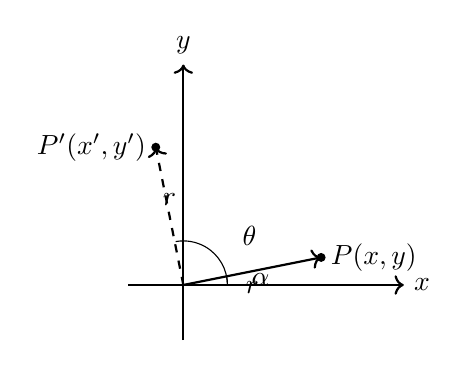
\begin{tikzpicture}[scale=0.7]
\draw[->,thick] (-1,0) -- (4,0) node[right]{$x$};
\draw[->,thick] (0,-1) -- (0,4) node[above]{$y$};
\filldraw (2.5,0.5) circle (2pt) node[right]{$P(x,y)$};
\filldraw (-0.5,2.5) circle (2pt) node[left]{$P'(x',y')$};
\draw[->,thick] (0,0) -- (2.5,0.5) node[midway,below]{$r$};
\draw[->,thick,dashed] (0,0) -- (-0.5,2.5) node[midway,above]{$r$};
\draw (0.8,0) arc (0:12:0.8);
\node at (1.4,0.1){$\alpha$};
\draw (0.8,0) arc (0:100:0.8);
\node at (1.2,0.9){$\theta$};
\end{tikzpicture}
\end{center}

\begin{exercise}
\item 用公式计算，不凭直觉：点$(3,0)$转$90^\circ$后到哪？转$270^\circ$后呢？
\item 用公式计算：点$(2,1)$转$180^\circ$后坐标是？
\item 用公式计算：点$(4,3)$转$90^\circ$后坐标是？
\item $\theta=45^\circ$时，计算$(1,0)$的像。($\cos45^\circ=\sin45^\circ=\frac{\sqrt2}{2}$)
\item 点$(1,1)$先转$90^\circ$，再对结果转$90^\circ$，再转$90^\circ$，再转$90^\circ$，写出每一步的坐标。旋转$360^\circ$后是否回到原位？用公式说明。
\item 写出点$(x,y)$绕原点顺时针旋转$90^\circ$（即$\theta=-90^\circ$）后的坐标。提示：$\cos(-90^\circ)=0$，$\sin(-90^\circ)=-1$。
\end{exercise}

\sectiontitle{1.3\quad 反射变换}

\textbf{定义}：设$l$是平面上一条直线。对于平面上任意一点$P$，过$P$作$l$的垂线，垂足为$H$。在射线$PH$的反向延长线上取一点$P'$，使得$HP' = PH$。则称点$P'$为点$P$关于直线$l$的反射像，这个对应关系称为关于$l$的反射变换（或轴对称变换），直线$l$称为对称轴。

简而言之：反射变换把一个点翻折到直线的另一侧，翻折前后该点到直线的距离不变，且连线垂直于对称轴。

\begin{center}
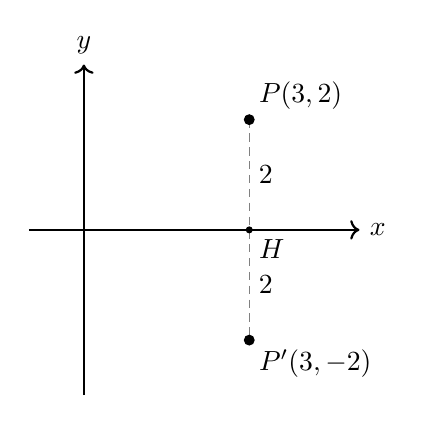
\begin{tikzpicture}[scale=0.7]
  \draw[->,thick] (-1,0) -- (5,0) node[right]{$x$};
  \draw[->,thick] (0,-3) -- (0,3) node[above]{$y$};
  \draw[densely dashed, gray] (3,2) -- (3,-2);
  \filldraw (3,2) circle (2.5pt) node[above right]{$P(3,2)$};
  \filldraw (3,-2) circle (2.5pt) node[below right]{$P'(3,-2)$};
  \filldraw (3,0) circle (1.5pt) node[below right]{$H$};
  \node at (3.3,1){$2$};
  \node at (3.3,-1){$2$};
\end{tikzpicture}
\end{center}

现在我们通过具体计算来看这个定义在坐标平面上怎么操作。先看关于$x$轴的反射。

\textbf{关于$x$轴的反射}：对称轴$l$是$x$轴（即直线$y=0$）。取点$P(3,2)$，它到$x$轴的距离是$|2|=2$。过$P$作$x$轴的垂线（竖直线$x=3$），垂足$H=(3,0)$。在$H$的另一侧取$P'$使$HP'=2$，即$P'=(3,-2)$。所以$(3,2)$关于$x$轴反射的像是$(3,-2)$。

再算几个：
\begin{itemize}
\item $(-1,4)$：到$x$轴距离$4$，垂线$x=-1$，垂足$(-1,0)$，反射像$(-1,-4)$。
\item $(5,0)$：到$x$轴距离$0$，点就在轴上，反射像就是它自己$(5,0)$。
\item $(2,-3)$：距离$3$，反射到轴上方$(2,3)$。
\end{itemize}

\begin{example}
从以上例子，归纳关于$x$轴反射的坐标规律。
\end{example}
\begin{solution}
每个点的$x$坐标完全不变，$y$坐标变成了它的相反数。规律是：
\[
x'=x,\quad y'=-y
\]
\end{solution}

\textbf{关于$y$轴的反射}：对称轴是$y$轴。用同样的方法分析：
\begin{itemize}
\item $(3,2)$：到$y$轴距离$3$，反射到$y$轴左侧$(-3,2)$。
\item $(5,-1)$：到$y$轴距离$5$，反射像$(-5,-1)$。
\item $(0,4)$：在$y$轴上，反射像$(0,4)$就是它自己。
\end{itemize}

\begin{example}
归纳关于$y$轴反射的坐标规律。
\end{example}
\begin{solution}
$y$坐标不变，$x$坐标取相反数：$x'=-x$，$y'=y$。
\end{solution}

\textbf{关于直线$y=x$的反射}：点$(3,2)$关于$y=x$的反射像是什么样子的？根据定义，$(3,2)$到直线$y=x$的垂线方程为$y-2=-(x-3)$，整理得$y=5-x$。这条垂线和$y=x$的交点（即垂足）是$(\frac52,\frac52)$。从$(3,2)$到垂足$(\frac52,\frac52)$的向量是$(-\frac12,\frac12)$，从垂足反方向走同样的距离，得到反射像$(2,3)$。

发现了吗？$(3,2)$关于$y=x$的反射像是$(2,3)$——就是把两个坐标对调了。再验证一个：$(4,1)$关于$y=x$的反射像应该是对调坐标得到$(1,4)$。我们来算：垂线$y-1=-(x-4)$交$y=x$于$(\frac52,\frac52)$，反射后确实是$(1,4)$。

继续验证：
\begin{itemize}
\item $(-1,3)$关于$y=x$反射：$(3,-1)$。
\item $(5,-2)$关于$y=x$反射：$(-2,5)$。
\end{itemize}

\begin{example}
归纳关于$y=x$反射的坐标规律。
\end{example}
\begin{solution}
$x$和$y$坐标互换：$x'=y$，$y'=x$。
\end{solution}

\textbf{关于直线$y=-x$的反射}：用同样的方法可以导出规律。$(3,2)$关于$y=-x$的反射像是$(-2,-3)$——坐标互换且都取相反数：
\[
x'=-y,\quad y'=-x
\]

最后注意一个性质：反复做两次同一个反射会回到原位。这是因为第一次反射把点翻到另一侧，第二次又翻回来了。你可以拿任何坐标验证：比如$(3,2)$关于$x$轴反射→$(3,-2)$→再反射一次→$(3,2)$。

\begin{exercise}
\item 点$(5,-3)$关于$x$轴对称后到哪？用$y$坐标取反的规则计算，然后画图验证。
\item 点$(-2,4)$关于$y$轴对称后到哪？
\item 分别计算$(4,1)$关于$y=x$和关于$y=-x$的反射像。
\item 点$A(2,3)$先关于$x$轴反射，再关于$y$轴反射，最终坐标是多少？这个结果相当于做了一个什么变换？提示：和$(2,3)$关于原点对称（即旋转$180^\circ$）的结果比较。
\item 点$B(1,0)$按照"关于$y=x$反射→关于$x$轴反射"的顺序做复合变换，写出每一步的坐标。
\end{exercise}

\sectiontitle{1.4\quad 伸缩变换}

\textbf{定义}：沿$x$轴方向拉伸$k$倍（$k\neq0$）的伸缩变换，是指把每个点的$x$坐标乘以$k$，$y$坐标保持不变。若$|k|>1$则拉长，$|k|<1$则缩短，$k<0$则拉伸到另一侧。

\begin{center}
\begin{tikzpicture}[scale=0.7]
  \draw[->,thick] (-1,0) -- (7,0) node[right]{$x$};
  \draw[->,thick] (0,-1) -- (0,5) node[above]{$y$};
  % Original square
  \draw[gray, thick, fill=lightblue!30] (0,0) rectangle (2,3);
  \node[gray] at (1,1.5){原正方形};
  % Stretched rectangle
  \draw[mainblue, thick] (0,0) rectangle (6,3);
  \node[mainblue] at (3,1.5){$k=3$拉伸后};
  \node at (3,-0.5){$x$方向拉伸$3$倍：$1\times1\to3\times1$};
\end{tikzpicture}
\end{center}

\begin{itemize}
\item $k=2$时：$(1,2)\to(2,2)$，$(3,1)\to(6,1)$，$(-1,3)\to(-2,3)$。注意$x$坐标都变成了原来的两倍。
\item $k=\frac12$时：$(4,3)\to(2,3)$，$(6,5)\to(3,5)$。$x$方向被压扁了一半。
\item $k=-2$时：$(1,2)\to(-2,2)$。$x$坐标不仅拉长了两倍，还翻到了$y$轴的另一边。
\end{itemize}

从这些例子归纳公式：$x'=kx$，$y'=y$。

同理，沿$y$轴方向拉伸$l$倍（$l\neq0$）：$x'=x$，$y'=ly$。

两个方向可以同时拉伸：$x'=kx$，$y'=ly$。

\begin{example}
举例：$k=2,l=3$时，$(1,1)$变成多少？原来的$1\times1$正方形变成了什么样的形状？面积变成了原来的几倍？
\end{example}
\begin{solution}
$(1,1)\to(2,3)$。正方形的四个顶点$(0,0),(1,0),(1,1),(0,1)$分别变成$(0,0),(2,0),(2,3),(0,3)$，是一个$2\times3$的矩形。面积$=2\times3=6$，是原来的$6$倍。
\end{solution}

\begin{exercise}
\item 计算：点$(4,5)$沿$x$方向拉伸$3$倍后到哪？沿$y$方向压缩到$\frac12$倍呢？
\item 点$(-2,5)$沿$x$方向拉伸$-1$倍，结果是什么？这和哪种变换效果相同？
\item $k=3,l=4$时，计算$(2,1)$的像。这个变换把面积放大了几倍？
\item 先沿$x$拉伸$2$倍，再沿$y$拉伸$3$倍。和先做$y$再做$x$的结果一样吗？取一个点算一下。
\item 沿$x$方向拉伸$2$倍后，能不能再做一个伸缩变换把图形恢复到原样？如果能，怎么做？
\end{exercise}

\sectiontitle{1.5\quad 投影变换}

\textbf{定义}：向$x$轴的投影变换，是指把每个点$(x,y)$映射为$(x,0)$。即保留横坐标，丢弃纵坐标。

\begin{itemize}
\item $(3,5)\to(3,0)$，$(3,-2)\to(3,0)$，$(-1,4)\to(-1,0)$。
\end{itemize}

注意，$(3,5)$和$(3,-2)$是两个完全不同的点，但它们的投影相同——都是$(3,0)$。这意味着从投影结果无法唯一确定原始的点。因此投影变换是不可逆的。

向$y$轴的投影：$x'=0$，$y'=y$。$(3,5)\to(0,5)$，$(-2,5)\to(0,5)$——$(-2,5)$和$(3,5)$投影后重合。

公式：
\begin{align*}
\text{向$x$轴投影}&: x'=x,\; y'=0\\
\text{向$y$轴投影}&: x'=0,\; y'=y
\end{align*}

\begin{example}
把单位正方形（顶点$(0,0),(1,0),(1,1),(0,1)$）分别向$x$轴和$y$轴投影。投影后的图形各是什么？
\end{example}
\begin{solution}
向$x$轴投影：四个顶点都变成$(0,0),(1,0),(1,0),(0,0)$——实际上退化为$x$轴上从$(0,0)$到$(1,0)$的线段。\\
向$y$轴投影：四个顶点变成$(0,0),(0,0),(0,1),(0,1)$——退化为$y$轴上从$(0,0)$到$(0,1)$的线段。
\end{solution}

\begin{exercise}
\item 点$(4,-3)$向$x$轴投影后到哪？向$y$轴投影后到哪？
\item 点$(2,5)$和$( -2,5)$向$y$轴投影后是否重合？$(2,5)$和$(2,-5)$向$x$轴投影后是否重合？
\item 为什么投影变换不可逆？从几何上说明。
\end{exercise}

\sectiontitle{1.6\quad 切变变换}

\textbf{定义}：沿$x$方向的切变变换（系数为$k$）是指把每个点$(x,y)$映射为$(x+ky,y)$。其中$y$坐标不变，$x$坐标上额外增加一个与$y$成正比的量。

试几个具体数字：
\begin{itemize}
\item $k=2$，点$(1,2)$：$x'=1+2\times2=5$，$y'=2$，变成$(5,2)$。
\item $k=2$，点$(3,0)$：$x'=3+2\times0=3$，$y'=0$，没变。因为$y=0$，不受切变影响。
\item $k=2$，点$(2,3)$：$x'=2+2\times3=8$，$y'=3$，变成$(8,3)$。
\item $k=-2$，点$(1,3)$：$x'=1+(-2)\times3=-5$，$y'=3$，变成$(-5,3)$。$k$为负时往左推。
\end{itemize}

把单位正方形做$k=1$的切变，看看形状怎么变。四个顶点：
\begin{align*}
A(0,0) &\to (0+1\times0,0)=(0,0)\\
B(1,0) &\to (1+1\times0,0)=(1,0)\\
C(1,1) &\to (1+1\times1,1)=(2,1)\\
D(0,1) &\to (0+1\times1,1)=(1,1)
\end{align*}
新顶点为$(0,0),(1,0),(2,1),(1,1)$——原来的正方形变成了一个平行四边形。注意底边长仍是$1$，高仍是$1$，所以面积没有变化。这是一个重要的性质，会在第三章中专门讨论。

\begin{center}
\begin{tikzpicture}[scale=1.2]
  \draw[->,thick] (-0.5,0) -- (3,0) node[right]{$x$};
  \draw[->,thick] (0,-0.5) -- (0,2) node[above]{$y$};
  % Original square
  \draw[gray, thick, dashed, fill=lightblue!20] (0,0) rectangle (1,1);
  \node[gray] at (0.5,0.5){正方形};
  % Sheared parallelogram
  \draw[mainblue, thick, fill=mainblue!10] (0,0) -- (1,0) -- (2,1) -- (1,1) -- cycle;
  \node[mainblue] at (1.2,0.4){平行四边形};
  \node at (1.2,-0.4){底$=1$，高$=1$，面积不变};
\end{tikzpicture}
\end{center}

\begin{exercise}
\item $k=3$时，计算$(1,2)$和$(1,0)$切变后的坐标。为什么$(1,0)$不变？
\item $k=-2$时，计算$(1,3)$切变后的坐标。负$k$意味着往哪个方向推？
\item 单位正方形的四个顶点做$k=3$的切变后，新顶点坐标各是什么？
\item 做一次$k=2$的切变后，再做一个什么参数的切变能把图形变回去？算一下验证。
\item 沿$y$方向的切变公式应该是怎样的？猜测并验证一个例子。
\end{exercise}

\sectiontitle{1.7\quad 本章小结}

我们已经见过五种变换：旋转、反射、伸缩、投影、切变。注意，每种变换的公式都写成
\[
x' = ax + by,\qquad y' = cx + dy
\]
的形式（平移是个例外，将在第五章处理）。它们的区别仅在于$a,b,c,d$分别取了什么数。

\begin{exercise}
\item 点$(3,4)$绕原点逆时针旋转$90^\circ$，再关于$x$轴反射。用每一步的公式计算最终坐标。
\item 点$(-1,5)$先关于$y=x$反射，再沿$x$方向拉伸$2$倍。写出每一步的坐标。
\item 点$(5,0)$做$x$方向$k=2$的切变，然后向$y$轴投影。最终坐标是什么？
\item 正方形顶点$(0,0),(2,0),(2,2),(0,2)$依次经过以下变换，逐步计算每个变换后的新顶点：\\
(a) 关于$x$轴反射\\
(b) 沿$y$方向拉伸$2$倍\\
(c) $x$方向$k=1$的切变\\
(d) 旋转$180^\circ$
\item 判断，并说明理由：\\
(a) 旋转变换保持两点间的距离不变吗？\\
(b) 投影变换可逆吗？\\
(c) 切变变换改变面积吗？\\
(d) 任何反射变换做两次等于恒等变换（什么都不变）吗？
\item 哪种变换能把正方形变成长方形？哪种能把正方形变成面积不变的平行四边形？
\item 思考：为什么线性变换的公式只能是$ax+by$而不能含$x^2$或$\sqrt{x}$？提示：直线经过这样的变换后，还应该是直线吗？
\end{exercise}

\sectiontitle{课后练习}

\subsection*{A组\quad 基础巩固}

\begin{exercise}
\item 点$(7,-2)$绕原点逆时针旋转$90^\circ$，求旋转后的坐标。
\item 点$(-4,6)$关于$x$轴对称后到哪？关于$y=x$对称后呢？
\item 点$(1.5,\,0)$做$x$方向拉伸$4$倍，再关于$y$轴对称，求最终坐标。
\item 点$(3,-1)$做$x$方向$k=-2$的切变，求变换后的坐标。向$x$轴投影后呢？
\item 单位正方形的四个顶点$(0,0),(1,0),(1,1),(0,1)$做旋转$270^\circ$，求四个新顶点坐标。
\item 点$A(2,5)$先旋转$180^\circ$，再关于$x$轴反射，再沿$x$方向拉伸$3$倍。求最终坐标。
\item 写出下列变换的公式：(a) 旋转$90^\circ$；(b) 关于$y=-x$反射；(c) $x$拉伸$\frac12$倍、$y$拉伸$3$倍。
\item 点$P$经旋转$90^\circ$后得到$(2,-3)$，求$P$的原坐标。
\item 判断下列变换是否可逆，并说明理由：旋转变换、向$x$轴投影、切变变换。
\item 一个点经三次关于$x$轴的反射，结果相当于做了什么变换？
\end{exercise}

\subsection*{B组\quad 挑战提升}

\begin{exercise}
\item 点$(1,\sqrt3)$绕原点逆时针旋转$30^\circ$，求旋转后的坐标。（提示：$\cos30^\circ=\frac{\sqrt3}{2}$，$\sin30^\circ=\frac12$。）
\item 写出关于直线$x=2$对称的变换公式。（提示：先平移坐标系把$x=2$变到$y$轴，反射，再平移回去——或者直接从定义推导。）
\item 旋转$\theta$后再旋转$-\theta$，结果回到了原位。用旋转公式代数验证这一点。
\item 两个旋转变换的复合：先旋转$\theta_1$再旋转$\theta_2$，总效果是什么？写出复合变换的坐标公式。
\item 能否找到两个不同的反射变换，它们的复合结果是一个旋转变换？如果能，写出具体的例子。
\item 某变换满足：$(1,0)\to(0,2)$，$(0,1)\to(-3,0)$，$(1,1)\to(-3,2)$。这个变换是哪种类型？写出它的公式。
\item 点$(3,5)$依次经过以下变换，求最终坐标：先绕原点逆时针旋转$135^\circ$，再关于$y=x$反射，最后沿$x$方向拉伸$\frac13$倍。\\
（提示：$\cos135^\circ=-\frac{\sqrt2}{2}$，$\sin135^\circ=\frac{\sqrt2}{2}$。）
\item 一个正方形顶点为$(0,0),(2,0),(2,2),(0,2)$，先做$x$方向$k=1.5$的切变，再绕原点旋转$45^\circ$。写出旋转后的四个顶点坐标（保留根号）。
\item 某点经过某种变换后到达$(5,-2)$。已知该变换是先沿$y$方向拉伸$3$倍，再关于直线$y=-x$反射。求原点的坐标。
\item 能否找到一个变换，它既不是单纯的旋转、反射、伸缩、投影、切变中的任何一种，但却是这五种中某两种的复合？举一个具体的坐标公式例子，并用一个点验证。
\end{exercise}

\newpage

\chaptertitle{第二章\quad 矩阵——变换的代码}

\sectiontitle{2.1\quad 把变换表示成一个方块}

回顾第一章的所有变换公式，它们有个共同的形式：
\[
x' = ax + by,\qquad y' = cx + dy
\]
每个具体的变换对应一组$(a,b,c,d)$。比如下面这些例子，你可以在第一章的公式中逐一验证：
\begin{align*}
\text{旋转}90^\circ &:a=0,\;b=-1,\;c=1,\;d=0\\
\text{关于$x$轴反射} &:a=1,\;b=0,\;c=0,\;d=-1\\
\text{$x$方向拉伸$3$倍} &:a=3,\;b=0,\;c=0,\;d=1\\
\text{向$x$轴投影} &:a=1,\;b=0,\;c=0,\;d=0\\
\text{$x$方向切变$k=2$} &:a=1,\;b=2,\;c=0,\;d=1
\end{align*}

既然每个变换只需要这四个数就能完全确定，把它们排成一个$2\times2$的方块比每次都写四个单独的数更方便。这个方块就叫\textbf{矩阵}：
\[
A = \begin{pmatrix}a&b\\c&d\end{pmatrix}
\]
左上角是$a$，右上角是$b$，左下角是$c$，右下角是$d$。

变换作用于点的计算，就是把列向量$\begin{pmatrix}x\\y\end{pmatrix}$左乘矩阵$A$来得到新坐标：
\[
\begin{pmatrix}x'\\y'\end{pmatrix}
= \begin{pmatrix}a&b\\c&d\end{pmatrix}
\begin{pmatrix}x\\y\end{pmatrix}
= \begin{pmatrix}ax+by\\cx+dy\end{pmatrix}
\]

操作就是：矩阵每一行的两个数分别与列向量的两个数相乘再相加。第一行乘出$x'$，第二行乘出$y'$。

\begin{example}
旋转$90^\circ$的矩阵是$\begin{pmatrix}0&-1\\1&0\end{pmatrix}$。用它来计算点$(3,2)$的旋转像：
\[
\begin{pmatrix}0&-1\\1&0\end{pmatrix}\begin{pmatrix}3\\2\end{pmatrix}
= \begin{pmatrix}0\times3+(-1)\times2\\1\times3+0\times2\end{pmatrix}
= \begin{pmatrix}-2\\3\end{pmatrix}
\]
结果$(-2,3)$。我们之前手动算过$(3,2)$旋转$90^\circ$的结果正是$(-2,3)$。
\end{example}

\begin{example}
伸缩矩阵$\begin{pmatrix}2&0\\0&3\end{pmatrix}$作用于点$(1,1)$：
\[
\begin{pmatrix}2&0\\0&3\end{pmatrix}\begin{pmatrix}1\\1\end{pmatrix}
= \begin{pmatrix}2\times1+0\times1\\0\times1+3\times1\end{pmatrix}
= \begin{pmatrix}2\\3\end{pmatrix}
\]
$x$被拉到$2$倍，$y$被拉到$3$倍。
\end{example}

\begin{example}
切变矩阵$\begin{pmatrix}1&2\\0&1\end{pmatrix}$作用于点$(1,2)$：
\[
\begin{pmatrix}1&2\\0&1\end{pmatrix}\begin{pmatrix}1\\2\end{pmatrix}
= \begin{pmatrix}1\times1+2\times2\\0\times1+1\times2\end{pmatrix}
= \begin{pmatrix}5\\2\end{pmatrix}
\]
$(1,2)$切变后变成$(5,2)$，和我们之前用手算的结果一致。
\end{example}

为了后面查阅方便，以下是第一章所有常见变换对应的矩阵：
\[
\begin{array}{c|c}
\text{变换} & \text{矩阵}\\\hline
\text{旋转$\theta$} & \begin{pmatrix}\cos\theta&-\sin\theta\\\sin\theta&\cos\theta\end{pmatrix}\\[2mm]
\text{关于$x$轴反射} & \begin{pmatrix}1&0\\0&-1\end{pmatrix}\\[2mm]
\text{关于$y$轴反射} & \begin{pmatrix}-1&0\\0&1\end{pmatrix}\\[2mm]
\text{关于$y=x$反射} & \begin{pmatrix}0&1\\1&0\end{pmatrix}\\[2mm]
\text{关于$y=-x$反射} & \begin{pmatrix}0&-1\\-1&0\end{pmatrix}\\[2mm]
\text{$x$方向拉伸$k$} & \begin{pmatrix}k&0\\0&1\end{pmatrix}\\[2mm]
\text{两方向拉伸$k,l$} & \begin{pmatrix}k&0\\0&l\end{pmatrix}\\[2mm]
\text{向$x$轴投影} & \begin{pmatrix}1&0\\0&0\end{pmatrix}\\[2mm]
\text{向$y$轴投影} & \begin{pmatrix}0&0\\0&1\end{pmatrix}\\[2mm]
\text{$x$方向切变$k$} & \begin{pmatrix}1&k\\0&1\end{pmatrix}
\end{array}
\]

\begin{exercise}
\item 用矩阵乘法计算：旋转$90^\circ$矩阵作用于$(5,0)$，写出运算过程。
\item 用矩阵乘法计算：关于$x$轴反射矩阵作用于$(-3,2)$。
\item 用矩阵乘法计算：$x$方向拉伸$4$倍矩阵作用于$(1,5)$。
\item 用矩阵乘法计算：$x$方向切变$k=3$矩阵作用于$(2,1)$。
\end{exercise}

\sectiontitle{2.2\quad 复合变换——两个动作连起来做}

我们来做两个具体的复合变换，用坐标直接算，观察结果。

\textbf{实验1：先旋转$90^\circ$，再关于$x$轴反射。}

取点$(1,2)$。先旋转$90^\circ$：$(1,2)\to(-2,1)$。再关于$x$轴反射：$(-2,1)\to(-2,-1)$。

现在换一个点$(3,0)$。旋转$90^\circ$：$(3,0)\to(0,3)$。再反射：$(0,3)\to(0,-3)$。

再试$(0,2)$。旋转$90^\circ$：$(0,2)\to(-2,0)$。反射：$(-2,0)\to(-2,0)$。

这三个复合变换的结果是$(-2,-1)$、$(0,-3)$、$(-2,0)$。有没有一个公式能一步算出复合效果？我们先把每一步的矩阵写出来：
\[
\text{旋转}90^\circ: R=\begin{pmatrix}0&-1\\1&0\end{pmatrix},\qquad
\text{反射}: S=\begin{pmatrix}1&0\\0&-1\end{pmatrix}
\]
我们想知道有没有一个矩阵$M$，使得$M$乘$(x,y)$直接得到先旋转后反射的结果。直觉上，这个$M$应该由$R$和$S$通过某种运算组合而成。

先算：$S$乘$R$（先旋转后反射，后做的写在前面）：
\[
SR = \begin{pmatrix}1&0\\0&-1\end{pmatrix}
\begin{pmatrix}0&-1\\1&0\end{pmatrix}
\]
计算每个位置：第一行第一列 $=1\times0+0\times1=0$；第一行第二列 $=1\times(-1)+0\times0=-1$；第二行第一列 $=0\times0+(-1)\times1=-1$；第二行第二列 $=0\times(-1)+(-1)\times0=0$。
\[
SR = \begin{pmatrix}0&-1\\-1&0\end{pmatrix}
\]
查一下第一章的表——这个矩阵对应的是关于$y=-x$的反射。

验证：用$SR$直接作用于$(1,2)$：
\[
\begin{pmatrix}0&-1\\-1&0\end{pmatrix}\begin{pmatrix}1\\2\end{pmatrix}
= \begin{pmatrix}-2\\-1\end{pmatrix}
\]
和我们分两步算的结果$(-2,-1)$一致！

\textbf{实验2：先关于$x$轴反射，再旋转$90^\circ$。}

把顺序反过来。先反射$S$后旋转$R$：
\[
RS = \begin{pmatrix}0&-1\\1&0\end{pmatrix}
\begin{pmatrix}1&0\\0&-1\end{pmatrix}
\]
第一行第一列 $=0\times1+(-1)\times0=0$；第一行第二列 $=0\times0+(-1)\times(-1)=1$；第二行第一列 $=1\times1+0\times0=1$；第二行第二列 $=1\times0+0\times(-1)=0$。
\[
RS = \begin{pmatrix}0&1\\1&0\end{pmatrix}
\]
这是关于$y=x$的反射。用$(1,2)$验证：$RS\cdot(1,2)^\text T$先反射得$(1,-2)$再旋转得$(2,1)$。$RS$直接乘：$(2,1)$。一致。

两个实验的结果不一样——$SR$给出关于$y=-x$的反射，$RS$给出关于$y=x$的反射。这说明\textbf{矩阵乘法的顺序一般不可交换}，$SR\neq RS$。

\textbf{实验3：先旋转$45^\circ$，再旋转$-45^\circ$。}

直觉：正转再反转，应该回到原位。用矩阵验证：
\[
R_{45}=\frac{\sqrt2}{2}\begin{pmatrix}1&-1\\1&1\end{pmatrix},\quad
R_{-45}=\frac{\sqrt2}{2}\begin{pmatrix}1&1\\-1&1\end{pmatrix}
\]
计算$R_{-45}R_{45}$：
\begin{align*}
&= \frac24\begin{pmatrix}1\cdot1+1\cdot1 & 1\cdot(-1)+1\cdot1\\ (-1)\cdot1+1\cdot1 & (-1)\cdot(-1)+1\cdot1\end{pmatrix}\\
&= \frac12\begin{pmatrix}2&0\\0&2\end{pmatrix}
= \begin{pmatrix}1&0\\0&1\end{pmatrix}
\end{align*}
结果是$\begin{pmatrix}1&0\\0&1\end{pmatrix}$，称为\textbf{单位矩阵}$I$。$I$作用于任何点都不改变它的位置。这里$R_{-45}R_{45}=I$说明正转反转互相抵消。

\textbf{实验4：两个伸缩。}

$A=\begin{pmatrix}2&0\\0&1\end{pmatrix}$（$x$拉伸2倍），$B=\begin{pmatrix}1&0\\0&3\end{pmatrix}$（$y$拉伸3倍）。

$AB=\begin{pmatrix}2&0\\0&3\end{pmatrix}$，$BA=\begin{pmatrix}2&0\\0&3\end{pmatrix}$。结果相同！为什么这次可以交换？因为两个方向各自独立拉伸，互不干扰。

通过以上四个实验，我们可以总结出矩阵乘法的规则：

\textbf{矩阵乘法的定义}：设$A=\begin{pmatrix}p&q\\r&s\end{pmatrix}$，$B=\begin{pmatrix}a&b\\c&d\end{pmatrix}$，定义它们的乘积（按$A$乘$B$的顺序）为：
\[
AB = \begin{pmatrix}p&q\\r&s\end{pmatrix}
\begin{pmatrix}a&b\\c&d\end{pmatrix}
= \begin{pmatrix}
pa+qc & pb+qd\\
ra+sc & rb+sd
\end{pmatrix}
\]
规则：前一行$\times$后一列，对应位置相乘再求和。

注意顺序：先做的变换写在右边，后做的写在左边。复合变换$BA$表示先做$A$再做$B$。

\begin{exercise}
\item 计算矩阵乘积：$\begin{pmatrix}2&1\\0&3\end{pmatrix}\begin{pmatrix}1&2\\3&4\end{pmatrix}$。写出每一步的计算过程。
\item 交换上题顺序：$\begin{pmatrix}1&2\\3&4\end{pmatrix}\begin{pmatrix}2&1\\0&3\end{pmatrix}$。结果相同吗？
\item 先旋转$180^\circ$再关于$x$轴反射，做矩阵乘法求复合矩阵。
\item 先关于$y=x$反射再旋转$90^\circ$，写出复合矩阵。
\item 验证伸缩矩阵$\begin{pmatrix}k&0\\0&l\end{pmatrix}$和$\begin{pmatrix}p&0\\0&q\end{pmatrix}$的乘法结果与顺序无关。
\item 计算$\begin{pmatrix}1&0\\0&0\end{pmatrix}\begin{pmatrix}0&0\\0&1\end{pmatrix}$（向$x$轴投影乘以向$y$轴投影）。这个结果代表什么变换？
\end{exercise}

\sectiontitle{2.3\quad 几个重要的特殊矩阵}

在计算矩阵乘法的过程中，有几类矩阵反复出现：

\textbf{单位矩阵} $I=\begin{pmatrix}1&0\\0&1\end{pmatrix}$。对任何点$(x,y)$，$I\cdot(x,y)^\text T=(x,y)^\text T$——这个变换什么都不做。对任何矩阵$A$，有$IA=AI=A$。$I$在矩阵乘法中的作用类似于数字$1$在普通乘法中的作用。

\textbf{零矩阵} $O=\begin{pmatrix}0&0\\0&0\end{pmatrix}$。任何点经过零矩阵都变成$(0,0)$。$OA=AO=O$。

\textbf{对角矩阵} $\begin{pmatrix}k&0\\0&l\end{pmatrix}$。非对角线位置全是$0$，主对角线上是两个伸缩系数。这类矩阵对应的变换是沿坐标轴方向的伸缩。当$k=l=1$时就是$I$。

\textbf{正交矩阵}：满足$A^\text T A=I$的方阵。旋转矩阵和反射矩阵都是正交矩阵。它们的共同特点是——作用后不改变向量的长度。

\begin{exercise}
\item 单位矩阵$I$的行列式（下章将定义）应该是什么？直觉上，$I$不改变面积。
\item 对角矩阵$\begin{pmatrix}k&0\\0&l\end{pmatrix}$何时可逆？何时不可逆？
\item 试写出一个不是旋转也不是反射的正交矩阵。
\end{exercise}

\sectiontitle{2.4\quad 解方程组与高斯消元法}

在许多实际问题中，我们知道的不是变换前的点，而是变换后的结果——即已知矩阵$A$和结果向量$\vec b$，要找到原来的点$\vec x$。这相当于解方程$A\vec x = \vec b$。

当矩阵是$2\times2$且$\det A\neq0$时，有个直接的办法——用逆矩阵（见2.5节）。但对于更大的矩阵或者含参数的方程，我们需要一个系统化的、一步步消去未知数的方法。这就是\textbf{高斯消元法}。

高斯消元法的核心思想是：通过三种合法的行变换，把增广矩阵$\begin{pmatrix}A & | & \vec b\end{pmatrix}$化为阶梯形，然后回代求解。三种行变换是：
\begin{enumerate}
\item 交换两行。
\item 某行乘以一个非零常数。
\item 某行的倍数加到另一行上。
\end{enumerate}

这三种操作都不会改变方程组的解。下面我们通过三种不同的结果情况来全面理解这个方法。

\vspace{0.2cm}
\noindent\textbf{情况一：唯一解}

\begin{example}
用高斯消元法解$\begin{cases}2x+3y=7\\x-2y=-4\end{cases}$。
\end{example}
\begin{solution}
增广矩阵：$\begin{pmatrix}2 & 3 & | & 7\\1 & -2 & | & -4\end{pmatrix}$

交换两行使第一行首项为$1$：$\begin{pmatrix}1 & -2 & | & -4\\2 & 3 & | & 7\end{pmatrix}$

$R_2$减去$R_1$的两倍：$\begin{pmatrix}1 & -2 & | & -4\\0 & 7 & | & 15\end{pmatrix}$

回代：从第二行得$7y=15$，即$y=15/7$。代入第一行：$x-2(15/7)=-4$，得$x=-4+30/7=2/7$。

解为$\begin{pmatrix}x\\y\end{pmatrix}=\begin{pmatrix}2/7\\15/7\end{pmatrix}$。
\end{solution}

\vspace{0.2cm}
\noindent\textbf{情况二：无穷多解}

\begin{example}
用高斯消元法解$\begin{cases}x+2y=3\\2x+4y=6\end{cases}$。
\end{example}
\begin{solution}
增广矩阵：$\begin{pmatrix}1 & 2 & | & 3\\2 & 4 & | & 6\end{pmatrix}$

$R_2\leftarrow R_2-2R_1$：$\begin{pmatrix}1 & 2 & | & 3\\0 & 0 & | & 0\end{pmatrix}$

第二行变成$0=0$——一个恒等式，不提供新的信息。第一个方程$x+2y=3$中有一个自由变量。取$y=t$（$t$为任意实数），则$x=3-2t$。

解为$\begin{pmatrix}x\\y\end{pmatrix}=\begin{pmatrix}3\\0\end{pmatrix}+t\begin{pmatrix}-2\\1\end{pmatrix}$（无穷多个解）。几何上，两个方程实际上是同一条直线。
\end{solution}

\vspace{0.2cm}
\noindent\textbf{情况三：无解}

\begin{example}
用高斯消元法解$\begin{cases}x+2y=3\\2x+4y=8\end{cases}$。
\end{example}
\begin{solution}
增广矩阵：$\begin{pmatrix}1 & 2 & | & 3\\2 & 4 & | & 8\end{pmatrix}$

$R_2\leftarrow R_2-2R_1$：$\begin{pmatrix}1 & 2 & | & 3\\0 & 0 & | & 2\end{pmatrix}$

第二行变成$0=2$——一个矛盾。无论$x$和$y$取什么值，都不可能满足这个等式。因此方程组无解。几何上，两个方程代表两条平行直线，永不相交。
\end{solution}

总结：高斯消元法有三种可能的输出结果——唯一解（系数矩阵可逆时）、无穷多解（方程数目不够时）、无解（出现矛盾时）。这三种情况囊括了所有线性方程组求解的可能。

\sectiontitle{2.5\quad 逆变换与逆矩阵}

如果矩阵$A$对应一个变换，这个变换把每个点$P$变到$P'$。有时候存在一个"反向"的变换，能把$P'$再变回$P$。这个反向的变换称为$A$的逆变换，对应的矩阵称为$A$的\textbf{逆矩阵}，记作$A^{-1}$。

\begin{example}
先看几个具体例子，从例子中观察规律。
\end{example}

\begin{solution}
(1) 旋转$90^\circ$的逆变换是旋转$-90^\circ$（顺时针转$90^\circ$）。我们已经验证过$R_{-90}R_{90}=I$，所以$R_{90}^{-1}=R_{-90}$。

(2) 反射的逆变换是它自己。因为反射做两次回到原位，$S^2=I$，所以$S^{-1}=S$。

(3) $x$方向拉伸$2$倍的逆变换是压缩到$\frac12$倍。

(4) 投影没有逆变换——因为不同点投影到同一个点，无法还原。
\end{solution}

对于一般的$2\times2$矩阵$A=\begin{pmatrix}a&b\\c&d\end{pmatrix}$，它的逆矩阵是：
\[
A^{-1} = \frac{1}{ad-bc}\begin{pmatrix}d&-b\\-c&a\end{pmatrix}
\]
分母上的$ad-bc$就是下一章要讲的行列式。如果$ad-bc=0$，这个分数就没有意义，对应的矩阵不可逆——几何上，这个变换把平面压扁了，信息丢失了，再也回不去了。

\begin{example}
求$A=\begin{pmatrix}2&3\\1&4\end{pmatrix}$的逆矩阵。
\end{example}
\begin{solution}
$ad-bc=2\times4-3\times1=5\neq0$。代入公式：
$A^{-1}=\frac15\begin{pmatrix}4&-3\\-1&2\end{pmatrix}$。
验证：$AA^{-1}=\frac15\begin{pmatrix}2&3\\1&4\end{pmatrix}\begin{pmatrix}4&-3\\-1&2\end{pmatrix}
=\frac15\begin{pmatrix}5&0\\0&5\end{pmatrix}=I$。
\end{solution}

逆矩阵的另一种理解方式是：解$A\vec x = \vec b$等价于$\vec x = A^{-1}\vec b$。这就是为什么上一节的高斯消元法和逆矩阵是同一问题的两个解法——高斯消元是通向解的路径，逆矩阵是把这条路径封装成的一个紧凑公式。

\sectiontitle{2.6\quad 从$2\times2$到$n\times n$}

矩阵的维度可以扩展到$n$。$3\times3$矩阵对应三维空间中的变换，$n\times n$矩阵对应$n$维空间中的变换。矩阵乘法、逆矩阵、高斯消元法的规则对任意大小都适用，只是数字多了而已。例如，$3\times3$矩阵乘法同样是"前行乘后列"：
\[
\begin{pmatrix}1&2&1\\3&0&2\\0&1&4\end{pmatrix}
\begin{pmatrix}2&0&1\\1&3&0\\0&1&2\end{pmatrix}
\]
每一项都是左行与右列的三对数字乘积之和。具体内容将在第四章中展开。

\sectiontitle{本章小结}

本章我们完成了从"几何变换"到"代数运算"的关键跨越。核心线索是：每种平面变换对应于一个$2\times2$矩阵，矩阵乘法正好对应变换的复合。矩阵乘法一般是不可交换的——先做A再做B与先做B再做A通常不同。在这套语言中，单位矩阵$I$扮演了"什么都不做"的角色，逆矩阵$A^{-1}$扮演了"撤销变换"的角色。最后，高斯消元法提供了解线性方程组的系统方法——有三种可能的结果：唯一解、无穷多解、无解。

\sectiontitle{课后练习}

\subsection*{A组\quad 基础巩固}

\begin{exercise}
\item 计算矩阵乘法，写出过程：$\begin{pmatrix}3&1\\2&5\end{pmatrix}\begin{pmatrix}1&0\\4&2\end{pmatrix}$。
\item 交换上题顺序：$\begin{pmatrix}1&0\\4&2\end{pmatrix}\begin{pmatrix}3&1\\2&5\end{pmatrix}$。结果相同吗？
\item 求$\begin{pmatrix}2&5\\1&3\end{pmatrix}$的逆矩阵（用公式$A^{-1}=\frac{1}{ad-bc}\begin{pmatrix}d&-b\\-c&a\end{pmatrix}$）。
\item 用高斯消元法解方程组：$\begin{cases}3x-2y=8\\x+4y=2\end{cases}$。写出增广矩阵的行变换过程。
\item 写出以下变换的矩阵：(a) 旋转$120^\circ$；(b) 关于$y=-x$反射后再旋转$90^\circ$的复合。
\item 计算：先$x$方向拉伸$2$倍再旋转$90^\circ$的复合矩阵。再交换顺序算一次。
\item 求矩阵$A=\begin{pmatrix}0&1\\1&0\end{pmatrix}$的$A^2$（即$A$乘$A$）。这个结果在几何上是什么意思？
\item 矩阵乘法是否满足结合律？即$(AB)C$是否等于$A(BC)$？任取三组数字验证。
\item 用高斯消元法解：$\begin{cases}2x+y-z=3\\x-2y+3z=1\\3x+y+2z=7\end{cases}$。
\item $\det(AB)=\det A\cdot\det B$。若$\det A=2$，$\det B=0.5$，则$\det(AB)$是多少？$\det(A^{-1})$呢？
\end{exercise}

\subsection*{B组\quad 挑战提升}

\begin{exercise}
\item 已知$AB=I$且$BA=I$，求证$A$和$B$互为逆矩阵。由此推导：若$AB=I$，是否一定有$BA=I$？（在方阵情况下是的，请说明理由。）
\item 求所有满足$A^2=I$的$2\times2$矩阵$A$。提示：有两类——反射类和对角线取$\pm1$类。
\item 用高斯消元法解以下含参数的方程组，讨论参数$a$取不同值时解的情况：$\begin{cases}x+ay=1\\ax+y=1\end{cases}$。
\item 若$A$是旋转矩阵，$B$是反射矩阵，$AB$还可以写成一个更简单的变换吗？试对几种具体角度列举复合结果。
\item 设$A=\begin{pmatrix}a&b\\c&d\end{pmatrix}$的一般逆矩阵为$\frac{1}{ad-bc}\begin{pmatrix}d&-b\\-c&a\end{pmatrix}$。如果$ad-bc=0$，逆矩阵不存在。从几何变换角度解释为什么。
\item 用高斯消元法解$\begin{cases}3x+2y=5\\\frac12 x-\frac13 y = 1\end{cases}$，写出增广矩阵和每一步行变换（允许使用分数）。
\item 求矩阵$A=\begin{pmatrix}\frac12&\frac{\sqrt3}{2}\\-\frac{\sqrt3}{2}&\frac12\end{pmatrix}$的逆矩阵。这个逆矩阵在几何上对应什么变换？与$A$的几何含义有何关系？
\item 计算乘积$\begin{pmatrix}\frac13&\frac23\\-\frac23&\frac13\end{pmatrix}\begin{pmatrix}\frac35&-\frac45\\\frac45&\frac35\end{pmatrix}$，并判断结果矩阵是否仍为正交矩阵。
\item 一个$3\times3$对角矩阵的对角元依次为$2,3,0$。它是否可逆？将$(x,y,z)$经此矩阵变换后的结果用坐标公式表示。哪些点会被压缩到同一点？
\end{exercise}

\newpage

\chaptertitle{第三章\quad 行列式——变换的放大倍率}

\sectiontitle{3.1\quad 二阶行列式——从平行四边形面积说起}

前两章我们一直在关注"每个点去了哪里"。现在换一个问题：经过一个变换之后，整个图形的面积是原来的多少倍？

考虑矩阵$A=\begin{pmatrix}a&b\\c&d\end{pmatrix}$。它把原来的基向量$(1,0)$变成$(a,c)$，把$(0,1)$变成$(b,d)$。原来边长为$1\times1$的正方形，经过$A$之后变成以$(a,c)$和$(b,d)$为两条邻边的平行四边形。

由向量$(a,c)$和$(b,d)$张成的平行四边形，其面积等于$|ad-bc|$。我们把这个数定义为矩阵$A$的行列式（determinant）：
\[
\det A = \begin{vmatrix}a&b\\c&d\end{vmatrix} = ad-bc
\]

\begin{center}
\begin{tikzpicture}[scale=0.8]
  \draw[->,thick] (-0.5,0) -- (5,0) node[right]{$x$};
  \draw[->,thick] (0,-0.5) -- (0,5) node[above]{$y$};
  % Unit square
  \draw[gray, thick, dashed, fill=lightblue!20] (0,0) -- (1,0) -- (1,1) -- (0,1) -- cycle;
  \node[gray] at (0.7,0.5){$1$};
  % Transformed vectors
  \draw[->, mainblue, very thick] (0,0) -- (3.5,1.2) node[midway, below]{$(a,c)$};
  \draw[->, mainblue, very thick] (0,0) -- (1.2,3.5) node[midway, left]{$(b,d)$};
  % Parallelogram
  \draw[mainblue, thick, fill=mainblue!10] (0,0) -- (3.5,1.2) -- (4.7,4.7) -- (1.2,3.5) -- cycle;
  \node[mainblue] at (2.5,2.8){面积$=|ad-bc|$};
\end{tikzpicture}
\end{center}

现在用这个公式逐一验证我们熟悉的变换，看行列式的值是否与我们直觉判断的面积倍数一致：

\textbf{验证1}：旋转$90^\circ$矩阵$\begin{pmatrix}0&-1\\1&0\end{pmatrix}$。$\det=0\times0-(-1)\times1=1$。从几何上，旋转$90^\circ$不改变正方形的大小和形状，面积不变，行列式$=1$合理。

\textbf{验证2}：$x$方向拉伸$3$倍$\begin{pmatrix}3&0\\0&1\end{pmatrix}$。$\det=3\times1-0\times0=3$。$1\times1$正方形变成了$3\times1$的矩形，面积确实是原来的$3$倍。

\textbf{验证3}：两方向分别拉伸$3$倍和$2$倍$\begin{pmatrix}3&0\\0&2\end{pmatrix}$。$\det=3\times2=6$。面积变成$6$倍。

\textbf{验证4}：$x$轴反射$\begin{pmatrix}1&0\\0&-1\end{pmatrix}$。$\det=1\times(-1)=-1$。绝对值$|-1|=1$，面积大小$1$倍（反射不改变面积）。但行列式多了一个负号。这个负号在下一节解释。

\textbf{验证5}：向$x$轴投影$\begin{pmatrix}1&0\\0&0\end{pmatrix}$。$\det=1\times0-0\times0=0$。正方形被压成线段，面积$=0$。

\textbf{验证6}：切变$\begin{pmatrix}1&2\\0&1\end{pmatrix}$。$\det=1\times1-2\times0=1$。切变把正方形变成平行四边形，但底和高都没变，面积不变——行列式$=1$。

\textbf{验证7}：旋转任意角度$\theta$：$\begin{pmatrix}\cos\theta&-\sin\theta\\\sin\theta&\cos\theta\end{pmatrix}$。
$\det=\cos^2\theta+\sin^2\theta=1$。不论$\theta$取多少，旋转不改变面积。

从以上七个验证中，行列式的几何含义已经非常清晰：行列式的绝对值$|\det A|$是变换将单位正方形面积放大或缩小的倍数。行列式为负表示定向反转，行列式为$0$表示图形被压扁降维。

\sectiontitle{3.2\quad 行列式为负——定向反转}

刚才$x$轴反射的行列式是$-1$，绝对值$|-1|=1$说明面积大小没变。负号在这里表示的是：变换把空间的"定向"反转了。

什么叫"定向"？在平面上，从$(1,0)$到$(0,1)$的旋转是逆时针的（这是标准的"右手方向"）。经过关于$x$轴的反射后，$(1,0)$仍是$(1,0)$，但$(0,1)$变成了$(0,-1)$——从$(1,0)$到$(0,-1)$的旋转方向变成了顺时针。这个坐标系手性的改变被行列式的负号捕捉住了。注意定向与单个向量的方向不同：旋转$180^\circ$把每个向量都反向，但$\det=(-1)\times(-1)=1$，它不改变手性（逆时针还是逆时针）。

一般规律：行列式为正时保持定向，行列式为负时反转定向。任何纯旋转变换的行列式恒为$1$，不反转定向。

\begin{exercise}
\item 关于$y$轴对称矩阵$\begin{pmatrix}-1&0\\0&1\end{pmatrix}$的行列式是多少？正还是负？
\item 旋转$180^\circ$矩阵$\begin{pmatrix}-1&0\\0&-1\end{pmatrix}$的行列式是多少？$180^\circ$旋转是否反转定向？为什么虽然每个向量都反向了，定向却没变？
\item 写出两个行列式为$-1$的矩阵（不能是题中已出现的）。
\end{exercise}

\sectiontitle{3.3\quad 行列式为$0$意味着什么？}

如果$\det A=0$，即$ad-bc=0$，也就是$ad=bc$，等价于$(a,c)$和$(b,d)$这两个列向量成比例。此时以它们为邻边的平行四边形退化成了线段，面积自然为$0$。但更深远的问题是：这个变换在几何上到底做了什么？为什么行列式为$0$的矩阵不可逆？

我们不要直接跳到抽象结论，而是一步一步从具体例子中归纳。

\vspace{0.2cm}
\noindent\textbf{实例1：投影矩阵。}
$A=\begin{pmatrix}1&0\\0&0\end{pmatrix}$，$\det=1\times0-0\times0=0$。

看两个列向量：第一个是$(1,0)$，第二个是$(0,0)$——零向量。第二个是第一个的$0$倍。这个矩阵把平面上的所有点都压到了$x$轴上：$(x,y)$变成$(x,0)$。无论$y$原来是多少，变换后$y'$恒为$0$。原来二维平面上的信息（$y$坐标）被完全丢失了。这就是为什么投影变换不可逆——你无法从$(x,0)$反推出原来的$y$是多少。

向$y$轴投影$\begin{pmatrix}0&0\\0&1\end{pmatrix}$同理：$\det=0$，列向量$(0,0)$和$(0,1)$中第一个是第二个的$0$倍。

\vspace{0.2cm}
\noindent\textbf{实例2：列向量成倍数。}
$B=\begin{pmatrix}2&4\\1&2\end{pmatrix}$，$\det=2\times2-4\times1=4-4=0$。

列向量：$(2,1)$和$(4,2)$。观察：$(4,2)=2\times(2,1)$——第二个列向量正好是第一个的$2$倍。它们指向同一个方向，共线。

用这个矩阵变换任意点$(x,y)$：$B\begin{pmatrix}x\\y\end{pmatrix}=\begin{pmatrix}2x+4y\\x+2y\end{pmatrix}$。注意第二个坐标恰好是第一个的一半：$(x+2y)=\frac12(2x+4y)$。所以变换后的所有像点都落在直线$y=\frac12 x$上。整个二维平面被压成了一条直线——原本分布在平面各处的点，现在全部挤在一条线上。

你在$(3,5)$和$(9,2)$两个不同的点分别算一下：前者变成$(2\cdot3+4\cdot5,\;1\cdot3+2\cdot5)=(26,13)$，后者变成$(2\cdot9+4\cdot2,\;1\cdot9+2\cdot2)=(26,13)$。居然重合了！无数个不同的原始点被映射到同一个像点。信息丢失了，逆矩阵不存在。

\vspace{0.2cm}
\noindent\textbf{实例3：再来一组不同的数。}
$C=\begin{pmatrix}3&6\\2&4\end{pmatrix}$，$\det=3\times4-6\times2=12-12=0$。

列向量：$(3,2)$和$(6,4)$。看到规律了吗？$(6,4)=2\times(3,2)$——又是第一个的倍数。这两个向量还是共线。用$C$作用在任何点上，像点都落在同一条直线上（通过原点、方向为$(3,2)$）。平面被压成了线。

\vspace{0.2cm}
\noindent\textbf{实例4：列向量不成比例的情况作对比。}
$D=\begin{pmatrix}2&3\\1&4\end{pmatrix}$，$\det=2\times4-3\times1=8-3=5\neq0$。

列向量：$(2,1)$和$(3,4)$。这次$(3,4)$不是$(2,1)$的倍数——无论你给$(2,1)$乘上什么数，都不可能得到$(3,4)$（因为乘$1.5$得$(3,1.5)$不是$(3,4)$；乘$2$得$(4,2)$也不是）。这两个向量不共线，它们指向不同的方向，张成了一个货真价实的平行四边形（面积$5$）。这个变换不会把平面压扁——它把平面映射到整个平面，每个像点唯一对应一个原像点。矩阵$D$是可逆的。

\vspace{0.2cm}
\noindent\textbf{归纳。}

上面四个实例揭示了同一个模式：当两个列向量不共线时（实例4），$\det\neq0$，变换保持平面的"二维性"，矩阵可逆。当两个列向量共线时（实例1-3）——即其中一个能够表示为另一个的倍数——$\det=0$，变换把平面压成了一维的直线（甚至一个点），无数不同的原像被映射到同一个像，矩阵不可逆。

这个关键概念有一个专门的名称。如果一组向量中存在某个向量能够表示为其他向量的线性组合（在二维中就是倍数关系），则称这组向量\textbf{线性相关}。反之，如果没有任何一个向量能表示为其他向量的线性组合（在二维中就是不共线），则称它们\textbf{线性无关}。

\textbf{行列式为$0$ $\Longleftrightarrow$ 列向量线性相关 $\Longleftrightarrow$ 变换降维（平面被压扁）$\Longleftrightarrow$ 矩阵不可逆。}

这组等价关系是学习后续章节的基础。记住它的几何图像：行列式不为零时，矩阵把正方形变成平行四边形；行列式为零时，矩阵把正方形压成一条线段——面积归零，信息丢失，再也回不去了。

\begin{exercise}
\item 判断矩阵$\begin{pmatrix}3&6\\2&4\end{pmatrix}$的两个列向量是否线性相关（是否共线），行列式是多少。
\item 矩阵$\begin{pmatrix}1&2\\0&0\end{pmatrix}$的行列式是多少？它的两个列向量线性相关吗？它把平面变成了什么？
\item 线性无关的两个向量在平面上的几何关系是什么？任写一个由线性无关列向量构成的$2\times2$矩阵。
\item 矩阵$\begin{pmatrix}1&0\\0&1\end{pmatrix}$是把平面压扁了吗？它的行列式是多少？可逆吗？
\end{exercise}

\sectiontitle{3.4\quad 三阶行列式与体积}

前面我们一直在二维平面上讨论：二阶行列式等于平行四边形的面积。现在自然要问：三维空间中的"体积放大倍率"该怎么算？这需要三阶行列式。我们同样不从公式出发，而是先看几个具体的三维变换，亲手算一算再总结。

\vspace{0.2cm}
\noindent\textbf{实例1：三方向伸缩。}

考虑一个$3\times3$对角矩阵：
\[
A = \begin{pmatrix}2&0&0\\0&3&0\\0&0&4\end{pmatrix}
\]
它把三维空间中的每个点$(x,y,z)$映射为$(2x,3y,4z)$。来算几个具体的点：
\begin{itemize}
\item $(1,0,0)$变成$(2,0,0)$——沿$x$轴拉长$2$倍。
\item $(0,1,0)$变成$(0,3,0)$——沿$y$轴拉长$3$倍。
\item $(0,0,1)$变成$(0,0,4)$——沿$z$轴拉长$4$倍。
\end{itemize}
原来$1\times1\times1$的单位立方体，三条棱分别被拉成了$2,3,4$。变成的长方体体积显然是$2\times3\times4=24$。直觉上，这个变换的体积放大倍率就是$24$。

\vspace{0.2cm}
\noindent\textbf{实例2：只改变一个方向。}

\[
B = \begin{pmatrix}1&0&0\\0&1&0\\0&0&5\end{pmatrix}
\]
只在$z$方向拉伸$5$倍，$x$和$y$方向不变。单位立方体变成底面$1\times1$、高$5$的柱体，体积$=5$。

\vspace{0.2cm}
\noindent\textbf{实例3：含切变的三维变换。}

\[
C = \begin{pmatrix}1&1&0\\0&1&1\\0&0&1\end{pmatrix}
\]
这个矩阵在$xy$平面内有切变（$x$受$y$影响），同时在$yz$平面内也有切变（$y$受$z$影响）。看几个具体的点：
\begin{itemize}
\item $(1,0,0)\to(1,0,0)$——$x$轴方向不变。
\item $(0,1,0)\to(1,1,0)$——$xy$平面内被斜推了。
\item $(0,0,1)\to(0,1,1)$——$z$方向的点被推到了$(0,1,1)$。
\end{itemize}
直觉上，切变只是"推了一把"，像推扑克牌一样——不改变体积。所以体积应该还是$1$。

\vspace{0.2cm}
\noindent\textbf{实例4：三维投影——压缩到平面上。}

\[
D = \begin{pmatrix}1&0&0\\0&1&0\\0&0&0\end{pmatrix}
\]
这个矩阵把每个点的$z$坐标清零：$(x,y,z)\to(x,y,0)$。整个三维空间被压扁到$xy$平面上——像用压路机把立方体碾成了薄片。体积自然为$0$。

\vspace{0.2cm}
\noindent\textbf{从实例到公式。}

上面四个例子中，我们靠直觉判断了体积变化。现在需要一套系统的方法——能对任意$3\times3$矩阵算出它的体积放大倍率（的绝对值）。这套方法就是三阶行列式。

三阶行列式是二阶行列式的自然延伸。展开规则是：
\[
\begin{vmatrix}
a_{11}&a_{12}&a_{13}\\
a_{21}&a_{22}&a_{23}\\
a_{31}&a_{32}&a_{33}
\end{vmatrix}
= a_{11}a_{22}a_{33}+a_{12}a_{23}a_{31}+a_{13}a_{21}a_{32}
-a_{13}a_{22}a_{31}-a_{12}a_{21}a_{33}-a_{11}a_{23}a_{32}
\]
记忆技巧：主对角线（左上→右下）方向的三项取正号，副对角线（右上→左下）方向的三项取负号。但初学时更可靠的做法是直接用公式逐项代入。

现在用公式验证我们的直觉判断：
\begin{itemize}
\item 实例1：$\det A=2\times3\times4=24$（只有主对角线乘积项非零）。$\checkmark$
\item 实例2：$\det B=1\times1\times5=5$（只有主对角线乘积）。$\checkmark$
\item 实例3：$\det C=1\times1\times1+1\times1\times0+0\times0\times0-0\times1\times0-1\times0\times1-1\times1\times0=1$。其他交叉项都含$0$，只剩$1$。$\checkmark$
\item 实例4：$\det D=1\times1\times0+0\times0\times0+0\times0\times0-0\times1\times0-0\times0\times0-1\times0\times0=0$。$\checkmark$
\end{itemize}

公式和直觉完全吻合。三阶行列式的绝对值就是三维变换的体积放大倍率，符号表达定向（三维中的手性）。

\vspace{0.2cm}
\noindent\textbf{从三维看线性相关。}

回顾3.3节：二维中，两个列向量共线（线性相关）$\Longleftrightarrow$ 行列式为$0$。在三维中，这个逻辑自然延伸到三个向量。

试一个例子：$E=\begin{pmatrix}1&0&1\\0&1&1\\0&0&0\end{pmatrix}$。第三个列向量$(1,1,0)$恰好等于前两个$(1,0,0)$和$(0,1,0)$的和——它可以被另外两个"表示"出来。算一下行列式：$\det E=1\times1\times0+\cdots=0$（第三行全零，行列式必为零）。

再看$F=\begin{pmatrix}1&2&3\\0&1&2\\0&0&0\end{pmatrix}$。第三行为零——意味着三个列向量的$z$分量全是$0$，它们全部躺在$xy$平面上。三个向量\textbf{共面}，张成的平行六面体厚度为零，体积为零，行列式为零。

归纳：在三维中，三个向量\textbf{线性相关}当且仅当它们共面——存在某个向量可以表示为另外两个的线性组合。此时行列式为$0$，矩阵不可逆（三维空间被压扁成二维平面甚至更低）。三个向量\textbf{线性无关}当且仅当它们不共面——真正在三个独立方向上撑开了空间，行列式不为零，矩阵可逆。

这一规律可以继续推广：在任意$n$维空间中，$n$个向量线性相关意味着它们被包含在一个低于$n$维的子空间内，行列式为零。

\begin{exercise}
\item 用展开公式计算$\begin{vmatrix}2&0&0\\0&3&0\\0&0&5\end{vmatrix}$。这个矩阵把体积放大了几倍？
\item 判断：若一个$3\times3$矩阵的三个列向量共面，它的行列式是多少？可逆吗？
\item 若一个$3\times3$矩阵的某两列恰好相等，行列式是多少？为什么？（提示：两列相等意味着什么线性关系？）
\end{exercise}

\sectiontitle{3.5\quad 行列式的核心性质}

二阶行列式的各种代数性质在更高阶中依然成立。和前面几节一样，我们先看具体的数字例子，再来总结每一条性质背后的几何意义。

\vspace{0.2cm}
\noindent\textbf{性质1：交换两行，行列式变号。}

取$A=\begin{pmatrix}2&1\\3&4\end{pmatrix}$，$\det A=2\times4-1\times3=5$。交换两行得$B=\begin{pmatrix}3&4\\2&1\end{pmatrix}$，$\det B=3\times1-4\times2=-5$。行列式从$5$变成了$-5$——绝对值没变，符号翻转。

几何上：交换两行相当于交换两个基向量在平行四边形中的顺序。原本从第一列到第二列是逆时针，交换后变成顺时针——定向反转了。

\vspace{0.2cm}
\noindent\textbf{性质2：某行乘$k$，行列式乘$k$。}

$A=\begin{pmatrix}2&1\\0&3\end{pmatrix}$，$\det A=2\times3=6$。把第一行乘$3$得$B=\begin{pmatrix}6&3\\0&3\end{pmatrix}$，$\det B=6\times3=18=3\times6$。

几何上：给某行乘$k$，相当于把那个方向的基向量拉伸了$k$倍，平行四边形的高（或底）变成了$k$倍，面积自然变成$k$倍。

同理，如果两行都翻倍，行列式变成$k^2$倍（每行独立贡献一个因子）。对$n$阶方阵，每行翻倍使行列式变成$k^n$倍。

\vspace{0.2cm}
\noindent\textbf{性质3：两行成比例，行列式为$0$。}

这一条我们已经反复见到。$A=\begin{pmatrix}1&2\\2&4\end{pmatrix}$，第二行恰好是第一行的$2$倍。$\det=1\times4-2\times2=0$。

也可以从3.3节的角度理解：两行成比例意味着两列也线性相关（在二阶中），平行四边形的两条邻边共线，面积为零。在高阶中，任意两行成比例都会导致行列式为零——因为它们对应的方向重合了。

\vspace{0.2cm}
\noindent\textbf{性质4：某行加上另一行的倍数，行列式值不变。}

$A=\begin{pmatrix}1&2\\3&4\end{pmatrix}$，$\det=1\times4-2\times3=-2$。将第一行的$2$倍加到第二行：$B=\begin{pmatrix}1&2\\3+2&4+4\end{pmatrix}=\begin{pmatrix}1&2\\5&8\end{pmatrix}$。$\det B=1\times8-2\times5=-2$。不变！

这个性质没有那么直观，但几何上的解释是：把一行的倍数加到另一行，在变换的视角下相当于在某个方向上叠加了一个切变操作。而切变（如1.6节所见）不改变平行四边形的底和高，因此面积不变。试试用$k=2$的切变矩阵$\begin{pmatrix}1&2\\0&1\end{pmatrix}$左乘$A$：结果矩阵的行列式是$\det A\times\det(\text{切变})=\det A\times1=\det A$。

\vspace{0.2cm}
\noindent\textbf{性质5：$\det(AB)=\det A\cdot\det B$。}

这可能是最重要的一条。先算两个具体矩阵各自的行列式和它们乘积的行列式：
\begin{align*}
A=\begin{pmatrix}2&0\\0&3\end{pmatrix},\;\det A&=6,\qquad
B=\begin{pmatrix}0&1\\1&0\end{pmatrix},\;\det B=-1\\[2pt]
AB=\begin{pmatrix}0&2\\3&0\end{pmatrix},\;\det(AB)&=0\times0-2\times3=-6=6\times(-1)=\det A\cdot\det B
\end{align*}

再试一组：$A$把面积放大$3$倍，$B$是投影矩阵（$\det B=0$）。那么$AB$：$\det(AB)=3\times0=0$。无论$A$怎么"放大"，只要$B$已经压扁了，复合结果还是扁的——$0$乘任何数还是$0$。

这个性质对数个变换的复合特别有用。比如三个矩阵连乘：$\det(ABC)=\det A\cdot\det B\cdot\det C$。特别地，逆矩阵的行列式：由$AA^{-1}=I$且$\det I=1$，得$\det A\cdot\det(A^{-1})=1$，即$\det(A^{-1})=1/\det A$。

下面把五条性质整理成一览表：

\[
\begin{array}{c|c}
\textbf{代数性质} & \textbf{几何意义}\\\hline
\text{交换两行，行列式变号} & \text{交换两个基向量的顺序，定向反转}\\
\text{某行乘$k$，行列式乘$k$} & \text{一个方向拉伸$k$倍，体积放大$k$倍}\\
\text{两行成比例，行列式为$0$} & \text{两个方向共线/共面，体积被压成$0$}\\
\text{某行加另一行的倍数，值不变} & \text{切变不改变体积——推一把不压缩}\\
\det(AB)=\det A\cdot\det B & \text{复合变换的放大倍率 $=$ 各自倍率相乘}
\end{array}
\]

这些性质不仅是行列式计算的口诀——每一条都对应着一个具体的几何动作。你可以在纸上画图验证，也可以在代数计算中反复应用。在后续各章中，它们会反复出现——尤其是 $\det(AB)=\det A\cdot\det B$ 在特征值和二次型的推导中是核心工具。

\sectiontitle{本章小结}

行列式是本书的第三块基石。它的几何含义极为直观：二阶行列式的绝对值 $=$ 平行四边形的面积，三阶行列式的绝对值 $=$ 平行六面体的体积。行列式的符号表示定向（手性是否反转），行列式为零表示变换降维（平面被压成线或点，空间被压成面）。其中最重要的等价关系是：$\det A=0 \Longleftrightarrow$ 列向量线性相关 $\Longleftrightarrow$ 变换降维 $\Longleftrightarrow A$ 不可逆。另外，行列式的五条代数性质（交换变号、行乘$k$则行列式乘$k$、成比例则为零、行加倍数不变、乘积的行列式$=$行列式的乘积）各有对应的几何解释——它们将在特征值、二次型等内容中反复出现。

\sectiontitle{课后练习}

\subsection*{A组\quad 基础巩固}
\begin{exercise}
\item 计算行列式并判断变换是放大还是缩小了面积（或改变了定向）：\\[2pt]
(a) $\begin{vmatrix}4&3\\1&2\end{vmatrix}$\quad
(b) $\begin{vmatrix}5&0\\0&7\end{vmatrix}$\quad
(c) $\begin{vmatrix}0&2\\3&0\end{vmatrix}$
\item 下列矩阵中哪些行列式为$0$？对于行列式为$0$的，判断两个列向量是否成比例：\\
(a) $\begin{pmatrix}1&2\\2&4\end{pmatrix}$\quad (b) $\begin{pmatrix}3&0\\0&-2\end{pmatrix}$\quad (c) $\begin{pmatrix}0&1\\-1&0\end{pmatrix}$
\item 计算$\begin{vmatrix}1&2&0\\0&3&1\\2&0&4\end{vmatrix}$。
\item 已知$\det A=3$，求$\det(2A)$（提示：$2A$相当于$A$的每一行都乘了$2$，行列式如何变化）。
\item 若$\det A=5$，$\det B=-2$，求$\det(AB)$和$\det(BA)$。
\item 矩阵$\begin{pmatrix}1&2\\3&4\end{pmatrix}$可逆吗？若可逆，求$\det(A^{-1})$。
\item 计算$\begin{vmatrix}x&1\\1&x\end{vmatrix}$，并求出使得行列式为$0$的$x$值。$x$取这些值时，两个列向量有什么关系？几何上发生了什么？
\item 用行列式性质判断：若一个$2\times2$矩阵的某一行全为零，其行列式是多少？为什么？
\item 计算对角矩阵$\begin{pmatrix}d_1&0&0\\0&d_2&0\\0&0&d_3\end{pmatrix}$的行列式。什么条件下这个矩阵不可逆？
\item 写出两个不同的$2\times2$矩阵，使得它们的行列式都为$0$，但列向量所沿的直线不同。
\end{exercise}

\subsection*{B组\quad 挑战提升}
\begin{exercise}
\item 三阶行列式中，若将第一列的$2$倍加到第三列，行列式值是否改变？用性质说明。
\item 证明：对于任何$2\times2$矩阵，$\det(A^2)=(\det A)^2$。并举出一个反例说明$\det(A^2)\neq\det A$一般不成立。
\item 计算：$\begin{vmatrix}a&b&c\\b&c&a\\c&a&b\end{vmatrix}$。提示：展开后尝试提取公因式，可分解为$(a+b+c)(a^2+b^2+c^2-ab-bc-ca)$。
\item 设$A$是斜对称矩阵（$A^{\text T}=-A$），且是奇数阶。证明$\det A=0$。提示：利用$\det(A^{\text T})=\det A$和$\det(-A)=(-1)^n\det A$。
\item 已知$\det\begin{pmatrix}2&3\\x&y\end{pmatrix}=1$，$\det\begin{pmatrix}1&4\\x&y\end{pmatrix}=2$。求$\det\begin{pmatrix}3&7\\x&y\end{pmatrix}$。提示：利用行列式关于列的线性性质，观察第三列与前两列的关系。
\item 计算$\begin{vmatrix}2&-1&3\\1&0&4\\-2&1&1\end{vmatrix}$。利用行变换简化计算（而非直接套展开公式）。
\item 设$A=\begin{pmatrix}k&2\\3&k\end{pmatrix}$。求使得$\det A=0$的所有$k$值。$k$取这些值时，$A$的列向量处于什么几何关系？
\item 计算$\begin{vmatrix}1&\frac12&\frac13\\\frac12&\frac13&\frac14\\\frac13&\frac14&\frac15\end{vmatrix}$。
\item 已知某$3\times3$矩阵的第三行是第一行的$2$倍减去第二行的$3$倍。不计算具体数字，判断该矩阵的行列式，并说明理由。
\end{exercise}

\newpage

\chaptertitle{第四章\quad 特征——变换的不变方向}

\sectiontitle{4.1\quad 观察：有没有方向特别"幸运"？}

前三章我们掌握了变换的两个基本侧面：矩阵告诉我们"每个点去了哪里"，行列式告诉我们"面积放大了几倍"。现在问一个更深层的问题：在变换中，有没有某些方向是"特殊"的——它们不偏不转，只是被拉长或缩短？如果有，怎么找到它们？这个问题将引向本书最核心的概念之一——特征值和特征向量。

对于大多数变换，随便选一个向量，经过变换后它的方向会偏转。但有些变换中存在一些特殊的向量——方向完全不偏，只是被拉长或被缩短了。

\textbf{例1}：伸缩变换$A=\begin{pmatrix}2&0\\0&3\end{pmatrix}$。
\begin{itemize}
\item $(1,0)$经过$A$变成$(2,0)$。方向还是水平，长度变成$2$倍。
\item $(0,1)$变成$(0,3)$。方向竖直不变，长度变成$3$倍。
\item 但斜方向的$(1,1)$变成$(2,3)$，方向明显变了——因为两个方向放大倍数不同。
\end{itemize}

\textbf{例2}：切变$A=\begin{pmatrix}1&2\\0&1\end{pmatrix}$。
\begin{itemize}
\item $(1,0)$经过$A$变成$(1,0)$——水平方向完全不变。
\item $(0,1)$变成$(2,1)$——方向变了。
\item $(2,1)$? 算一下：$(2,1)$在切变下变成$(2+2,1)=(4,1)$。方向变了。
\end{itemize}

\textbf{例3}：旋转$90^\circ$。不管选什么方向，转了$90^\circ$肯定变了——所以旋转没有任何这样的"幸运方向"。

\begin{center}
\begin{tikzpicture}[scale=0.85]
  \draw[->,thick] (-0.5,0) -- (4,0) node[right]{$x$};
  \draw[->,thick] (0,-0.5) -- (0,4) node[above]{$y$};
  % Eigenvector direction 1: horizontal → stays horizontal, stretched
  \draw[->, mainblue, very thick] (0,0) -- (1,0) node[midway, below]{$\vec v_1$};
  \draw[->, mainblue, very thick, dashed] (0,0) -- (2,0) node[near end, above]{$2\vec v_1$};
  % Eigenvector direction 2: vertical → stays vertical, stretched
  \draw[->, mainblue, very thick] (0,0) -- (0,1) node[midway, left]{$\vec v_2$};
  \draw[->, mainblue, very thick, dashed] (0,0) -- (0,3) node[near end, right]{$3\vec v_2$};
  % Non-eigenvector: (1,1) → (2,3) direction changes
  \draw[->, gray, thick] (0,0) -- (1,1) node[midway, above left]{$\vec w$};
  \draw[->, gray, thick, dashed] (0,0) -- (2,3) node[right]{$A\vec w$};
  \node at (2,-0.7){伸缩变换：特征方向保持不偏，斜方向偏转};
\end{tikzpicture}
\end{center}

这些不改变方向、只改变长度的向量，被称为\textbf{特征向量}。长度改变的比例，被称为这个特征向量对应的\textbf{特征值}。

\begin{exercise}
\item 对于伸缩矩阵$A=\begin{pmatrix}4&0\\0&0.5\end{pmatrix}$，凭直觉判断：$(1,0)$和$(0,1)$是不是特征向量？如果是，对应的特征值是多少？
\item 在例2的切变矩阵$\begin{pmatrix}1&2\\0&1\end{pmatrix}$中，沿$x$轴方向的向量是否总是特征向量？沿$y$轴方向的呢？
\item 为什么旋转变换没有实特征向量？从几何直觉和代数计算两个角度简答。
\end{exercise}

\sectiontitle{4.2\quad 怎么找特征值和特征向量？}

条件就是$A\vec v = \lambda\vec v$。移项得$(A-\lambda I)\vec v = 0$。要使这个方程有非零解$\vec v$（$\vec v\neq\vec 0$），矩阵$(A-\lambda I)$的行列式必须为零——因为若行列式不为零，矩阵可逆，方程$(A-\lambda I)\vec v=0$两边左乘逆矩阵后只能得到$\vec v = \vec 0$。因此特征值$\lambda$必须满足：
\[
\det(A-\lambda I) = 0
\]
这就是\textbf{特征方程}。对$2\times2$矩阵$A=\begin{pmatrix}a&b\\c&d\end{pmatrix}$：
\[
\begin{vmatrix}a-\lambda & b\\c & d-\lambda\end{vmatrix}
= \lambda^2-(a+d)\lambda+(ad-bc) = 0
\]
解出$\lambda$之后代回$(A-\lambda I)\vec v=0$，就能求出对应的特征向量。

\begin{example}
求$A=\begin{pmatrix}2&0\\0&3\end{pmatrix}$的特征值和特征向量。
\end{example}
\begin{solution}
特征方程：$\begin{vmatrix}2-\lambda&0\\0&3-\lambda\end{vmatrix}=(2-\lambda)(3-\lambda)=0$，得$\lambda_1=2$，$\lambda_2=3$。

$\lambda_1=2$：$(A-2I)\vec v=\begin{pmatrix}0&0\\0&1\end{pmatrix}\begin{pmatrix}x\\y\end{pmatrix}=0$，得$y=0$，$x$任意。特征向量形如$(t,0)$——即所有水平方向的向量。

$\lambda_2=3$：$(A-3I)\vec v=\begin{pmatrix}-1&0\\0&0\end{pmatrix}\begin{pmatrix}x\\y\end{pmatrix}=0$，得$x=0$，$y$任意。特征向量形如$(0,t)$——所有竖直方向的向量。
\end{solution}

\begin{example}
求$A=\begin{pmatrix}2&1\\1&2\end{pmatrix}$的特征值和特征向量。
\end{example}
\begin{solution}
特征方程：$\begin{vmatrix}2-\lambda&1\\1&2-\lambda\end{vmatrix}=(2-\lambda)^2-1=\lambda^2-4\lambda+3=0$。

$\lambda_1=1$：$(A-I)\vec v=\begin{pmatrix}1&1\\1&1\end{pmatrix}\begin{pmatrix}x\\y\end{pmatrix}=0$，得$x+y=0$，$\vec v_1=(1,-1)$。

$\lambda_2=3$：$(A-3I)\vec v=\begin{pmatrix}-1&1\\1&-1\end{pmatrix}\begin{pmatrix}x\\y\end{pmatrix}=0$，得$x-y=0$，$\vec v_2=(1,1)$。

结论：沿$(1,-1)$方向拉伸$1$倍（即不变），沿$(1,1)$方向拉伸$3$倍。
\end{solution}

\begin{exercise}
\item 求$\begin{pmatrix}5&0\\0&2\end{pmatrix}$的特征值和特征向量。
\item 求$\begin{pmatrix}1&2\\2&1\end{pmatrix}$的特征值和特征向量。
\item 旋转$180^\circ$矩阵$\begin{pmatrix}-1&0\\0&-1\end{pmatrix}$有特征向量吗？特征值是多少？
\item 已知$\det A=6$，$\tr A=5$（迹$=a+d$），求特征值。
\end{exercise}

\sectiontitle{4.3\quad 旋转为什么没有实特征向量？}

旋转$90^\circ$矩阵$A=\begin{pmatrix}0&-1\\1&0\end{pmatrix}$。特征方程：$\lambda^2+1=0$，$\lambda=\pm i$——没有实根。

这从几何上完全说得通：旋转$90^\circ$把每个非零向量都转了方向，不存在任何"方向不变"的向量。如果特征方程只有复数根而没有实数根，说明矩阵含有旋转的成分。

\begin{exercise}
\item 旋转$60^\circ$矩阵的特征方程是否有实数根？用$\cos60^\circ=\frac12$、$\sin60^\circ=\frac{\sqrt3}{2}$代入特征方程验证。
\item 一个矩阵的特征方程为$\lambda^2+4=0$。这个矩阵可能代表什么类型的变换？为什么？
\end{exercise}

\sectiontitle{4.4\quad 特征值的和与积}

从4.2节的特征方程出发，我们可以发现一个优雅的关系。对$2\times2$矩阵$A=\begin{pmatrix}a&b\\c&d\end{pmatrix}$，特征方程为：
\[
\lambda^2-(a+d)\lambda+(ad-bc)=0
\]
由韦达定理（一元二次方程的根与系数的关系），两根之和为一次项系数的相反数，两根之积为常数项。因此：
\[
\lambda_1+\lambda_2 = a+d = \tr A,\qquad
\lambda_1\lambda_2 = ad-bc = \det A
\]
这里$\tr A = a+d$（主对角线元素之和）称为矩阵的\textbf{迹}（trace）。

这两个公式极为有用——它们把特征值、行列式、迹这三个看似独立的概念串联在了一起：
\begin{itemize}
\item $\det A=0$ $\Longleftrightarrow$ 至少有一个特征值为$0$ $\Longleftrightarrow$ 存在一个方向被压缩消失（降维）。这与第三章的结论完全呼应。
\item $\tr A=0$ $\Longleftrightarrow$ 两个特征值互为相反数。
\end{itemize}

更妙的是，这组关系不限于二阶——对任意$n\times n$矩阵，始终有：
\[
\lambda_1+\lambda_2+\cdots+\lambda_n = \tr A,\qquad
\lambda_1\lambda_2\cdots\lambda_n = \det A
\]
特征值之和总是等于迹（所有主对角线元素之和），特征值之积总是等于行列式。这是线性代数中最优美的恒等式之一——它意味着，即使你无法一眼看出$n$个特征值各自是多少，你也能立刻知道它们的和与积。

\begin{example}
已知$\det A=12$，$\tr A=7$，求$A$的两个特征值。
\end{example}
\begin{solution}
$\lambda_1+\lambda_2=7$，$\lambda_1\lambda_2=12$。联立解：$(\lambda-3)(\lambda-4)=0$，得$\lambda_1=3,\lambda_2=4$。
\end{solution}

\begin{example}
若$\det A=0$且$\tr A=5$，特征值是多少？
\end{example}
\begin{solution}
$\lambda_1+\lambda_2=5$，$\lambda_1\lambda_2=0$。必有一个特征值为$0$，另一个为$5$。$\det=0$意味着矩阵不可逆，有一个方向被压缩消失——特征值$0$正好反映了这一点。
\end{solution}

\begin{exercise}
\item 已知$\det A=-6$，$\tr A=1$，求$A$的两个特征值。
\item 若$\det A=0$，能否唯一确定两个特征值？如果还知道$\tr A=4$呢？
\end{exercise}

\sectiontitle{4.5\quad 施密特正交化——扶正坐标系}

有时我们找到的几个向量并不互相垂直，但在很多应用（如下一章的二次型）中，我们需要一组互相垂直的坐标系。施密特正交化的作用就是：给定一组线性无关的向量，构造出一组互相垂直的向量，且它们张成同一个空间。

给定$\vec v_1,\vec v_2$：
\begin{align*}
\vec u_1 &= \vec v_1\\
\vec u_2 &= \vec v_2 - \frac{\vec v_2\cdot\vec u_1}{\vec u_1\cdot\vec u_1}\,\vec u_1
\end{align*}
几何意义：先取$\vec v_1$作为第一个正交方向$\vec u_1$；然后从$\vec v_2$中减去它在$\vec u_1$上的投影分量，剩下的部分必然垂直于$\vec u_1$——这就是$\vec u_2$。

\begin{example}
$\vec v_1=(1,1)$，$\vec v_2=(1,2)$，做施密特正交化。
\end{example}
\begin{solution}
$\vec u_1=(1,1)$。$\vec v_2$在$\vec u_1$上的投影长度$=\frac{(1,2)\cdot(1,1)}{(1,1)\cdot(1,1)}=\frac{3}{2}$。

$\vec u_2=(1,2)-\frac32(1,1)=(-\frac12,\frac12)$。

验证：$\vec u_1\cdot\vec u_2=1\cdot(-\frac12)+1\cdot\frac12=0$，垂直。
\end{solution}

\begin{exercise}
\item 对$\vec v_1=(3,0)$和$\vec v_2=(0,4)$做施密特正交化。结果说明了什么？
\item 对$\vec v_1=(1,2)$和$\vec v_2=(3,4)$做施密特正交化，并验证结果是否垂直。
\end{exercise}

\sectiontitle{4.6\quad 对角化——在最自然的坐标系下看变换}

如果矩阵$A$有$n$个线性无关的特征向量，以它们为列排成矩阵$P$，则：
\[
A = PDP^{-1},\qquad D = \begin{pmatrix}\lambda_1&0\\0&\lambda_2\end{pmatrix}
\]
在特征向量构成的新坐标系下，变换就简单了——它只是沿着每个特征方向做伸缩而已。$P^{-1}AP=D$这个等式叫对角化：把坐标系换到特征方向上之后，矩阵变成了对角形。

我们通过一个完整的例子走一遍全过程。

\begin{example}
对$A=\begin{pmatrix}2&1\\1&2\end{pmatrix}$做对角化。
\end{example}
\begin{solution}
我们已经知道$A$的特征值为$\lambda_1=1$（特征向量$\vec v_1=(1,-1)$）和$\lambda_2=3$（特征向量$\vec v_2=(1,1)$）。

第1步：将特征向量作为列向量排成矩阵$P$：
\[
P = \begin{pmatrix}1&1\\-1&1\end{pmatrix}
\]

第2步：求$P$的逆矩阵。$\det P = 1\times1-1\times(-1)=2$，所以
\[
P^{-1} = \frac12\begin{pmatrix}1&-1\\1&1\end{pmatrix}
\]

第3步：验证$P^{-1}AP$是否等于对角阵：
\begin{align*}
P^{-1}AP &= \frac12\begin{pmatrix}1&-1\\1&1\end{pmatrix}
\begin{pmatrix}2&1\\1&2\end{pmatrix}
\begin{pmatrix}1&1\\-1&1\end{pmatrix}\\[1mm]
&= \frac12\begin{pmatrix}1&-1\\3&3\end{pmatrix}
\begin{pmatrix}1&1\\-1&1\end{pmatrix}
= \frac12\begin{pmatrix}2&0\\0&6\end{pmatrix}
= \begin{pmatrix}1&0\\0&3\end{pmatrix}
\end{align*}
结果正是以特征值为对角元的对角矩阵。$\checkmark$

这告诉我们：在$P$的列向量$(1,-1)$和$(1,1)$构成的新坐标系中，$A$这个变换就只是一个沿两个方向分别拉伸$1$倍和$3$倍的简单伸缩。
\end{solution}

注意：不是所有矩阵都能对角化。例如$A=\begin{pmatrix}1&1\\0&1\end{pmatrix}$只有一个特征值$\lambda=1$（二重）和一个特征方向$(1,0)$，无法拼出可逆矩阵$P$。这表明该矩阵除了伸缩还含有切变的成分，不能简化为纯伸缩。后续课程中会系统分析这类情况。

\begin{exercise}
\item 对$\vec v_1=(2,1)$和$\vec v_2=(1,3)$做施密特正交化。
\item 对角矩阵$\begin{pmatrix}3&0\\0&5\end{pmatrix}$的特征值和特征向量是什么？
\item 如果$\det A=0$，$A$可能有多少个特征值为$0$？
\end{exercise}

\sectiontitle{本章小结}

特征值和特征向量是本书的第四块基石。核心方程 $A\vec v=\lambda\vec v$ 刻画了变换中方向不变、仅被拉伸的特殊向量。特征值之和等于迹、之积等于行列式——这组关系将特征值与前面各章的概念完美串联。当矩阵拥有足够多线性无关的特征向量时，可以通过 $P^{-1}AP=D$ 对角化——这意味着在特征向量构成的坐标系中，变换简化为了纯伸缩。施密特正交化则提供了将任意一组向量"扶正"为垂直坐标系的方法，为后续二次型的处理做准备。旋转没有实特征向量这一事实，也从代数上印证了几何直觉：旋转改变了所有方向。

\sectiontitle{课后练习}

\subsection*{A组\quad 基础巩固}
\begin{exercise}
\item 求下列矩阵的特征值和特征向量：\\
(a) $\begin{pmatrix}4&1\\2&3\end{pmatrix}$\quad (b) $\begin{pmatrix}3&0\\0&3\end{pmatrix}$\quad (c) $\begin{pmatrix}0&1\\1&0\end{pmatrix}$
\item 求$\begin{pmatrix}2&1\\2&3\end{pmatrix}$的特征值和特征向量。
\item 已知$\det A=8$，$\tr A=6$，求$A$的两个特征值。
\item 判断矩阵$\begin{pmatrix}3&1\\0&3\end{pmatrix}$的特征值情况。它是一个对角的倍数加切变，特征向量有什么特点？
\item 已知某$2\times2$矩阵的特征值为$2$和$-1$，对应的特征向量分别为$(1,0)$和$(1,1)$。求出该矩阵。（提示：利用$A=PDP^{-1}$。）
\item 矩阵$\begin{pmatrix}2&1\\0&2\end{pmatrix}$的特征值是多少？它的特征向量有什么几何意义？
\item 对$\vec v_1=(3,0)$和$\vec v_2=(1,2)$做施密特正交化。
\item 编写一个$2\times2$矩阵，使得其特征值乘积为$6$，特征值和为$5$。
\end{exercise}

\subsection*{B组\quad 挑战提升}
\begin{exercise}
\item 若$A$的特征值为$\lambda_1,\lambda_2$，求证$A^{-1}$的特征值为$1/\lambda_1,1/\lambda_2$。$A^{-1}$的特征向量是否与$A$相同？
\item 若$\lambda$是$A$的特征值，则$\lambda^2$是$A^2$的特征值。验证此结论并用两个具体例子检验。
\item 证明：若$A$可逆，则$A$和$A^{-1}$有相同的特征向量。
\item 已知某矩阵的特征值为$2$和$-3$，求$A^2-2A+I$的特征值。
\item 设$A$是二阶斜对称矩阵（对角全为$0$）。求$A$的特征值，并验证它们是否为实数。
\item 求$A=\begin{pmatrix}1&4\\2&3\end{pmatrix}$的特征值与特征向量。这两个特征向量是否正交？如果否，对它们做施密特正交化。
\item 矩阵$A=\begin{pmatrix}0&2\\-1&3\end{pmatrix}$的特征值是否为实数？若非实数，说明$A$的几何含义中含有什么成分。
\item 对于一个$2\times2$矩阵，已知$\det A=-2$且$\tr A=0$。不计算具体矩阵，求其特征值，并判断该变换是否可能是一个旋转。
\item 对$\vec v_1=(1,3)$和$\vec v_2=(2,-1)$做施密特正交化。验证结果是否正交，并说明为什么这里施密特正交化后得到的向量方向与原始向量不同（与课后练习A组第7题作对比）。
\end{exercise}

\newpage

\chaptertitle{第五章\quad 齐次坐标与仿射变换}

\sectiontitle{5.1\quad 平移——一个无法用$2\times2$矩阵表示的变换}

前四章我们学习的所有变换都能写成$x'=ax+by$，$y'=cx+dy$。但有一个最常见的操作——平移$(x,y)\to(x+a,y+b)$——上面这种形式写不出来。

为什么呢？因为平移在$x'$和$y'$的表达式里各多了一个常数项$a$和$b$。标准形式$x'=ax+by$要求$x'$是$x$和$y$的线性组合，不能有游离的常数。这暴露出一个基本限制：平移改变了原点，而线性变换（$ax+by$型）把原点固定在原处。平移后原点$(0,0)$去了$(a,b)$，不再是原点了。

为了把平移也统一进矩阵的框架，需要一个巧妙的办法。

\begin{exercise}
\item 验证：以下变换中哪些保持原点$(0,0)$不动？(a) 旋转$90^\circ$；(b) 平移$(2,-1)$；(c) 关于$x$轴反射；(d) 向右平移$3$再旋转$180^\circ$。
\item 为什么"保持原点不动"是能用$2\times2$矩阵表示的变换的必要条件？
\end{exercise}

\sectiontitle{5.2\quad 齐次坐标——给平面加一个维度}

我们不把平面上的点记作$(x,y)$，而是记作$(x,y,1)$。多出来的第三个坐标$"1"$只是一个占位符，不表示任何真实的空间方向，唯一的作用是让平移可以被"装"进矩阵乘法。

在齐次坐标下，向右平移$3$、向上平移$2$的操作写成：
\[
\begin{pmatrix}1&0&3\\0&1&2\\0&0&1\end{pmatrix}
\begin{pmatrix}x\\y\\1\end{pmatrix}
= \begin{pmatrix}x+3\\y+2\\1\end{pmatrix}
\]
你看，第一行把$x$坐标加了$3$，第二行加了$2$，第三行保持不变。平移就这样被$3\times3$矩阵表达出来了。

所有的$2\times2$线性变换（旋转、反射、拉伸、切变）在齐次坐标下也扩充为$3\times3$矩阵——只需把$2\times2$部分放在左上角，第三行第三列写$1$，其余位置写$0$：
\[
\begin{pmatrix}a&b&0\\c&d&0\\0&0&1\end{pmatrix}
\]

\begin{example}
将先沿$x$方向拉伸$2$倍，再向右平移$3$，用齐次坐标一步算出$(1,2)$的像。
\end{example}
\begin{solution}
线性部分$A=\begin{pmatrix}2&0\\0&1\end{pmatrix}$，平移$(3,0)$。
齐次矩阵：$\begin{pmatrix}2&0&3\\0&1&0\\0&0&1\end{pmatrix}$。
作用于$(1,2)$：$\begin{pmatrix}2\cdot1+0\cdot2+3\cdot1\\0\cdot1+1\cdot2+0\cdot1\\1\end{pmatrix}=\begin{pmatrix}5\\2\\1\end{pmatrix}$，即$(5,2)$。
\end{solution}

\begin{example}
用齐次坐标计算：先关于$x$轴反射，再平移$(-1,4)$，求点$(2,3)$的像。
\end{example}
\begin{solution}
反射矩阵$\begin{pmatrix}1&0\\0&-1\end{pmatrix}$，平移$(-1,4)$。齐次矩阵为：
\[
\begin{pmatrix}1&0&-1\\0&-1&4\\0&0&1\end{pmatrix}
\]
作用于$(2,3)$：$\begin{pmatrix}1\cdot2+0\cdot3+(-1)\cdot1\\0\cdot2+(-1)\cdot3+4\cdot1\\1\end{pmatrix}=\begin{pmatrix}1\\1\\1\end{pmatrix}$，即$(1,1)$。
\end{solution}

\begin{exercise}
\item 用齐次坐标计算：先旋转$90^\circ$再平移$(2,0)$，求点$(1,3)$的像。
\item 写出纯平移$(a,b)$的$3\times3$齐次坐标矩阵的一般形式。
\item 若一个$3\times3$齐次坐标矩阵的第三行不是$(0,0,1)$，它还能表示平面上的仿射变换吗？试分析。
\end{exercise}

\sectiontitle{5.3\quad 仿射变换的一般形式}

在齐次坐标下，一个任意仿射变换的矩阵长这样：
\[
\begin{pmatrix}
a&b&t_x\\
c&d&t_y\\
0&0&1
\end{pmatrix}
\]
左上角的$2\times2$子矩阵$A$是线性部分（旋转、反射等），右上角的$(t_x,t_y)$是平移部分。仿射变换就是"先线性变换，再平移"的总和。

按线性部分$A$的性质，可以给仿射变换分类。下面逐一用具体矩阵验证每类的特点。

\textbf{第一类：刚体运动。}$A$是正交矩阵，即$A^{\text T}A=I$，例如旋转矩阵或反射矩阵。此时$|\det A|=1$。

举个具体例子：$A=\begin{pmatrix}0&-1\\1&0\end{pmatrix}$（旋转$90^\circ$），$\vec t=(3,2)$。对应的$3\times3$齐次矩阵为$\begin{pmatrix}0&-1&3\\1&0&2\\0&0&1\end{pmatrix}$。这个变换先绕原点旋转$90^\circ$再向右上平移——相当于把一个图形在平面上刚性搬动。因为旋转不改变两点间的距离（$|A\vec v|=|\vec v|$对所有$\vec v$成立），平移也不改变距离，所以整个变换保持所有点间距离不变，面积绝对值也不变（$|\det A|=1$）。

\textbf{第二类：相似变换。}$A=kR$，其中$R$是旋转矩阵，$k>0$是缩放因子。例如$A=\begin{pmatrix}2&0\\0&2\end{pmatrix}$（整体放大$2$倍），$\vec t=(1,0)$。这个变换保持形状——原来的正方形放大后还是正方形，原来的圆放大后还是圆——只是大小变了。面积放大倍率为$|\det A|=k^2=4$。

\textbf{第三类：一般仿射变换。}$A$是任意可逆矩阵，例如$A=\begin{pmatrix}2&1\\0&3\end{pmatrix}$（含切变和不等比例伸缩）。$\vec t$任意。这类变换不保持角度和长度，但保持一个重要的几何性质：平行线在变换后仍然是平行线（你可以验证：两条原本平行的直线在$A$的作用下仍然平行，因为线性变换保持向量的线性关系）。

\textbf{第四类：降维变换。}$\det A=0$。例如$A=\begin{pmatrix}1&0\\0&0\end{pmatrix}$（向$x$轴投影），$\vec t$任意。整个平面被压扁到一条直线上，再平移——结果仍然是一条直线。这类变换不可逆，面积归零。

\sectiontitle{5.4\quad 变换的分解与复合}

任何一个仿射变换都可以唯一地分解为：先做线性部分$A$，再做平移$\vec t$。也可以反过来先平移再线性变换，这两种分解给出不同的矩阵表示，但都是同一个变换。

两个仿射变换的复合仍然是一个仿射变换。在齐次坐标中，复合就是矩阵乘法，非常方便。

\begin{example}
求两个仿射变换的复合：先做$T_1$（向右平移$2$），再做$T_2$（旋转$90^\circ$）。写出复合变换的齐次坐标矩阵，并计算点$(1,0)$的像。
\end{example}
\begin{solution}
$T_1$的矩阵：$\begin{pmatrix}1&0&2\\0&1&0\\0&0&1\end{pmatrix}$，$T_2$的矩阵：$\begin{pmatrix}0&-1&0\\1&0&0\\0&0&1\end{pmatrix}$。

复合（先$T_1$后$T_2$，$T_2$在前）：$T_2T_1=\begin{pmatrix}0&-1&0\\1&0&0\\0&0&1\end{pmatrix}\begin{pmatrix}1&0&2\\0&1&0\\0&0&1\end{pmatrix}=\begin{pmatrix}0&-1&0\\1&0&2\\0&0&1\end{pmatrix}$。

作用于$(1,0)$：$\begin{pmatrix}0&-1&0\\1&0&2\\0&0&1\end{pmatrix}\begin{pmatrix}1\\0\\1\end{pmatrix}=\begin{pmatrix}0\\3\\1\end{pmatrix}$，即$(0,3)$。

验证：先平移$(1,0)\to(3,0)$，再旋转$90^\circ$得$(0,3)$，一致。
\end{solution}

\begin{exercise}
\item 直接用齐次坐标矩阵乘法验证：先旋转$90^\circ$再向右平移$2$，与先平移$2$再旋转$90^\circ$，复合结果不同。指出两个复合变换分别把原点$(0,0)$变到了哪里——为什么不同？
\end{exercise}

\sectiontitle{本章小结}

仿射变换统一了线性变换和平移。核心技巧是齐次坐标——给平面上的点多加一维$(x,y,1)$，从而把平移"装进"$3\times3$矩阵的右上角。这使得旋转+平移（刚体运动）、伸缩+平移（相似变换）以及任意线性变换+平移都可以统一用$3\times3$矩阵表达和复合。按线性部分$A$的行列式，可以区分保持面积（$|\det A|=1$）、缩放面积（$|\det A|\neq1$）和降维（$\det A=0$）三类仿射变换。这套语言在计算机图形学中用来表达所有二维图形的移动、旋转和缩放。

\sectiontitle{课后练习}

\subsection*{A组\quad 基础巩固}
\begin{exercise}
\item 用齐次坐标矩阵计算：点$(2,3)$平移$(1,-2)$后的坐标。
\item 写出以下变换的$3\times3$齐次坐标矩阵：\\
(a) 先绕原点旋转$45^\circ$再向右平移$5$个单位；\\
(b) 先向$x$轴投影再向下平移$3$个单位。
\item 一个仿射变换的$3\times3$矩阵为$\begin{pmatrix}3&0&2\\0&2&1\\0&0&1\end{pmatrix}$。这个变换对点$(1,1)$作用后坐标是多少？它把面积放大了几倍？（提示：面积倍率只看线性部分$A$的$|\det A|$。）
\item 判断以下仿射变换是否保持面积：旋转+平移；投影+平移；切变+平移；反射+平移。
\item 写出先关于$x$轴对称再平移$(0,-2)$的齐次坐标矩阵，并计算$(3,4)$的像。
\end{exercise}

\subsection*{B组\quad 挑战提升}
\begin{exercise}
\item 一个仿射变换把$(0,0)$变成$(1,2)$，把$(1,0)$变成$(4,2)$，把$(0,1)$变成$(1,5)$。求出它的$3\times3$齐次坐标矩阵。
\item 二维平移矩阵是$3\times3$的，那么三维平移矩阵是几阶的？它长什么样？
\item 证明：两个刚体运动的复合仍然是刚体运动。
\item 一个仿射变换把$(0,0)$映射到$(2,-1)$，把$(1,0)$映射到$(5,1)$，把$(0,1)$映射到$(0,3)$。求该变换的$3\times3$齐次矩阵，并将它分解为"线性部分+平移部分"。
\item 用齐次坐标验证：先绕原点旋转$60^\circ$再向右平移$4$个单位的变换，与先向右平移$4$个单位再绕原点旋转$60^\circ$的变换，结果不同。写出两者的$3\times3$矩阵，并分别计算它们将$(1,1)$映射到了哪里（保留根号）。
\item 在计算机图形学中，一个矩形窗口的四个角点坐标为$(0,0),(3,0),(3,2),(0,2)$。若先将其绕自身中心旋转$180^\circ$再整体向右平移$5$个单位，写出对应的$3\times3$齐次矩阵并求变换后的四个角点坐标。
\end{exercise}

\newpage

\chaptertitle{第六章\quad 二次型——用矩阵研究圆锥曲线}

前面五章，我们逐一建立了矩阵、行列式、特征值、齐次坐标这四块基石。这一章，我们将把它们全部用上——来优雅地解决一个经典几何问题：如何判断一个含有$xy$交叉项的二次曲线到底是椭圆、双曲线还是抛物线？你会发现，答案就藏在特征值的正负号里。这是全书的高潮，也是你检验自己是否真正掌握了前五章的最佳时刻。

\sectiontitle{6.1\quad 一个问题：为什么有些曲线是"歪"的？}

在解析几何中，椭圆的标准方程是$\frac{x^2}{a^2}+\frac{y^2}{b^2}=1$，双曲线是$\frac{x^2}{a^2}-\frac{y^2}{b^2}=1$。它们的对称轴都和坐标轴对齐，形状很"正"。

但实际问题中，圆锥曲线往往长这样：
\[
5x^2+4xy+2y^2=1,\qquad
x^2-4xy+y^2=1
\]
这些方程里出现了一项$xy$——交叉项。交叉项让曲线"歪"了，使得它的主轴不再和坐标轴对齐。怎么判断这些"歪"曲线到底是椭圆、双曲线还是抛物线？传统做法是先旋转坐标系消掉$xy$项，再分类。过程繁琐。

有了矩阵之后，这个问题有了一个简洁的解法。

\begin{exercise}
\item 下列方程中哪些含有交叉项$xy$？哪些没有？\\
(a) $2x^2+3y^2=5$\quad (b) $x^2-2xy+y^2=0$\quad (c) $4x^2-y^2=1$\quad (d) $x^2+3xy+2y^2=4$
\item 对于不含交叉项的方程，你能直接判断曲线类型吗？(a)和(c)各是什么类型？
\end{exercise}

\sectiontitle{6.2\quad 从例子出发：怎么把$xy$项拆进矩阵}

看一个具体的二次型：$5x^2+4xy+2y^2$。把它写成矩阵形式：
\[
5x^2+4xy+2y^2=
\begin{pmatrix}x&y\end{pmatrix}
\begin{pmatrix}5&2\\2&2\end{pmatrix}
\begin{pmatrix}x\\y\end{pmatrix}
\]

注意$xy$的系数$4$被平均分到了两个非对角线位置（各放$2$），保持矩阵对称。展开验证一下：第一行乘列向量得$5x+2y$，再左乘行向量得$(x,y)$与$(5x+2y,2x+2y)$的内积，即$x(5x+2y)+y(2x+2y)=5x^2+4xy+2y^2$，正确。

一般地，二次型$ax^2+2bxy+cy^2$对应的对称矩阵是：
\[
M = \begin{pmatrix}a&b\\b&c\end{pmatrix}
\]
注意$xy$的系数写成了$2b$，这样$b$恰好分到两个非对角位置。如果原方程是$ax^2+pxy+cy^2$的形式，则$b=p/2$。

再看一个例子：$x^2-4xy+y^2$对应的矩阵是$\begin{pmatrix}1&-2\\-2&1\end{pmatrix}$——把$-4xy$的系数$-4$平分到两个非对角位置各$-2$。

\begin{exercise}
\item 写出以下二次型的对称矩阵：\\
(a) $x^2+6xy+9y^2$\quad (b) $2x^2-2xy+y^2$\quad (c) $x^2+y^2$
\item 验证：将你的答案代入$\begin{pmatrix}x&y\end{pmatrix}M\begin{pmatrix}x\\y\end{pmatrix}$，展开后是否得到原二次型。
\end{exercise}

\sectiontitle{6.3\quad 核心发现：特征值直接消掉交叉项}

现在做一件关键的事。把坐标轴转一个角度$\theta$，新旧坐标的关系是：
\[
\begin{pmatrix}x\\y\end{pmatrix}
= \begin{pmatrix}\cos\theta&-\sin\theta\\\sin\theta&\cos\theta\end{pmatrix}
\begin{pmatrix}X\\Y\end{pmatrix}
\]
代入二次型，经过旋转后$XY$项的系数变为$0$——这意味着在新的坐标系中曲线不再"歪"。留下来的表达式会变成什么样子？我们不看公式推导，直接用几个例子来发现规律。

\vspace{0.2cm}
\noindent\textbf{实例1：}$5x^2+4xy+2y^2$。对应矩阵$M=\begin{pmatrix}5&2\\2&2\end{pmatrix}$。先求$M$的特征值：
\[
\det(M-\lambda I)=\begin{vmatrix}5-\lambda&2\\2&2-\lambda\end{vmatrix}=\lambda^2-7\lambda+6=0,\quad\lambda_1=6,\;\lambda_2=1.
\]
如果做坐标旋转，$XY$项被消掉后，留下的标准形恰好是$6X^2+Y^2$。因此$5x^2+4xy+2y^2=1$化为$6X^2+Y^2=1$——一个椭圆。

\vspace{0.2cm}
\noindent\textbf{实例2：}$x^2-4xy+y^2$。对应矩阵$M=\begin{pmatrix}1&-2\\-2&1\end{pmatrix}$。特征值：
\[
\det(M-\lambda I)=\begin{vmatrix}1-\lambda&-2\\-2&1-\lambda\end{vmatrix}=\lambda^2-2\lambda-3=0,\quad\lambda_1=3,\;\lambda_2=-1.
\]
旋转后标准形为$3X^2-Y^2$。方程$x^2-4xy+y^2=1$化为$3X^2-Y^2=1$——一个双曲线。

\vspace{0.2cm}
\noindent\textbf{实例3：}再取一个例子来确认这个规律。$3x^2+2xy+3y^2$。对应矩阵$M=\begin{pmatrix}3&1\\1&3\end{pmatrix}$。
\[
\det(M-\lambda I)=(3-\lambda)^2-1=\lambda^2-6\lambda+8=0,\quad\lambda_1=4,\;\lambda_2=2.
\]
旋转后标准形为$4X^2+2Y^2$。方程$3x^2+2xy+3y^2=4$化为$4X^2+2Y^2=4$，即$\frac{X^2}{1}+\frac{Y^2}{2}=1$——还是一个椭圆，但长短轴比例不同。

\vspace{0.2cm}
\noindent\textbf{归纳。}

三个例子揭示了一个统一的规律：每个二次型经过坐标旋转化为标准形$\lambda_1X^2+\lambda_2Y^2$之后，系数$\lambda_1$和$\lambda_2$恰好就是对称矩阵$M$的两个特征值。这不是巧合——数学上可以严格证明，旋转后的$XY$项系数消去的条件，恰好等价于特征方程（详见进阶教材）。但从使用者的角度，你只需要记住这一条：

\textbf{结论：不需要做坐标旋转变换，直接求$M$的特征值，标准形就出来了。}

\begin{exercise}
\item 写出$3x^2+2xy+3y^2$的对称矩阵，求特征值，并由此判断$3x^2+2xy+3y^2=4$的曲线类型。
\item 为什么判断曲线类型只需要特征值而不需要实际做坐标旋转？用两三句话解释核心原理。
\end{exercise}

\sectiontitle{6.4\quad 用特征值分类圆锥曲线}

三个实例涵盖了三种曲线类型，这不是偶然。我们先用更多的例子确认这个模式，再总结分类规则。

\vspace{0.2cm}
\noindent\textbf{例A（两个正特征值）：}$2x^2+4xy+5y^2=9$。$M=\begin{pmatrix}2&2\\2&5\end{pmatrix}$，$\lambda_1=6$，$\lambda_2=1$。两特征值都为正——椭圆。

\vspace{0.2cm}
\noindent\textbf{例B（一正一负）：}$x^2-6xy+y^2=1$。$M=\begin{pmatrix}1&-3\\-3&1\end{pmatrix}$，特征方程$\lambda^2-2\lambda-8=0$，$\lambda_1=4$，$\lambda_2=-2$。一正一负——双曲线。

\vspace{0.2cm}
\noindent\textbf{例C（一个特征值为零）：}$4x^2+12xy+9y^2=1$。$M=\begin{pmatrix}4&6\\6&9\end{pmatrix}$，$\lambda_1=13$，$\lambda_2=0$。有一个零特征值——抛物线。

\vspace{0.2cm}
\noindent\textbf{例D（两个相等的正特征值）：}$x^2+y^2=4$。$M=\begin{pmatrix}1&0\\0&1\end{pmatrix}$，$\lambda_1=\lambda_2=1$。两特征值相等且为正——圆（椭圆的特例）。

这四个例子加上6.3节的三个，共七条曲线，它们的特征值符号和曲线类型的对应关系没有丝毫例外。我们可以安全地归纳出以下分类规则：

\[
\begin{array}{c|c}
\textbf{特征值符号} & \textbf{曲线类型}\\\hline
\lambda_1,\lambda_2>0\;\text{或}\;<0 & \text{椭圆（$\lambda_1=\lambda_2$时为圆）}\\
\lambda_1>0,\lambda_2<0\;\text{或反之} & \text{双曲线}\\
\lambda_1\lambda_2=0\;\text{（一个为零）} & \text{抛物线}
\end{array}
\]

注意$\lambda_1\lambda_2=\det M$。因此$\det M>0$对应椭圆，$\det M<0$对应双曲线，$\det M=0$对应抛物线——与解析几何中的判别式$ac-b^2$等价（实际上$\det M = ac-b^2$），但矩阵的解释更直接：$\det M$是特征值的乘积，它的符号直接告诉我们特征值的正负号分布。

\begin{example}
判断$4x^2+12xy+9y^2=1$的曲线类型。
\end{example}
\begin{solution}
$M=\begin{pmatrix}4&6\\6&9\end{pmatrix}$。特征方程$\lambda^2-13\lambda=0$，得$\lambda_1=13$，$\lambda_2=0$。
有一个特征值为$0$，这是\textbf{抛物线}。
\end{solution}

\begin{exercise}
\item 不计算特征值，仅凭$\det M$的符号判断以下曲线的类型：\\
(a) $2x^2+4xy+5y^2=9$\quad (b) $x^2-6xy+9y^2=1$\\
提示：$\det M = ac-b^2$。
\item 若$\det M=0$，为什么曲线一定是抛物线（或退化为两条直线/一个点）？从特征值和降维两个角度解释。
\end{exercise}

\sectiontitle{6.5\quad 主轴方向——特征向量告诉你曲线怎么摆}

知道了曲线类型之后，下一个问题是：它的主轴（长轴和短轴，或实轴和虚轴）沿着什么方向？答案仍然在特征向量里。

以$5x^2+4xy+2y^2=1$为例，我们已经知道$\lambda_1=6$，$\lambda_2=1$。下面找出主轴方向。

\begin{example}
求椭圆$5x^2+4xy+2y^2=1$的长短轴方向。
\end{example}
\begin{solution}
第1步：对$\lambda_1=6$求特征向量。$(M-6I)\vec v=\begin{pmatrix}-1&2\\2&-4\end{pmatrix}\begin{pmatrix}x\\y\end{pmatrix}=0$。
由第一行$-x+2y=0$得$\vec v_1$沿$(2,1)$方向。

第2步：对$\lambda_2=1$求特征向量。$(M-I)\vec v=\begin{pmatrix}4&2\\2&1\end{pmatrix}\begin{pmatrix}x\\y\end{pmatrix}=0$。
由第一行$4x+2y=0$得$\vec v_2$沿$(1,-2)$方向。

第3步：这两个特征向量互相垂直（验证：$(2,1)\cdot(1,-2)=0$），分别就是椭圆的两条主轴的方向。

第4步：判断长轴对应哪个特征值。旋转后的标准方程为$6X^2+Y^2=1$，即$\frac{X^2}{1/6}+\frac{Y^2}{1}=1$。半轴长为$1/\sqrt{6}\approx0.41$和$1$。$Y$方向半轴更长，所以长轴沿$\lambda_2=1$对应的特征向量方向$(1,-2)$，短轴沿$\lambda_1=6$对应的特征向量方向$(2,1)$。

\begin{center}
\begin{tikzpicture}[scale=0.65]
  \draw[->,thick] (-3,0) -- (3,0) node[right]{$x$};
  \draw[->,thick] (0,-3) -- (0,3) node[above]{$y$};
  \draw[->, mainblue, very thick] (0,0) -- (2,1) node[above right]{$Y$（长轴）};
  \draw[->, mainblue, very thick] (0,0) -- (-1,2) node[above left]{$X$（短轴）};
  \draw[->, mainblue, very thick] (0,0) -- (-2,-1);
  \draw[->, mainblue, very thick] (0,0) -- (1,-2);
  \draw[thick, mainblue!60!black] plot[smooth cycle, tension=0.8] coordinates {
    (1,-1.85) (1.22,-1.5) (1.8,-0.8) (2,-0.3) (1.9,0.3) (1.6,1) (1,1.5) (0.5,1.8)
    (-0.3,2) (-1,1.8) (-1.5,1.5) (-1.85,0.8) (-1.9,0) (-1.7,-0.8) (-1.2,-1.5) (-0.5,-1.9)
  };
  \node at (0,-3.2){$5x^2+4xy+2y^2=1$——倾斜椭圆及其主轴};
\end{tikzpicture}
\end{center}
\end{solution}

\begin{example}
求双曲线$x^2-4xy+y^2=1$的实轴和虚轴方向。
\end{example}
\begin{solution}
$M=\begin{pmatrix}1&-2\\-2&1\end{pmatrix}$，特征值$\lambda_1=3$，$\lambda_2=-1$。

$\lambda_1=3$：$(M-3I)\vec v=\begin{pmatrix}-2&-2\\-2&-2\end{pmatrix}\begin{pmatrix}x\\y\end{pmatrix}=0$，得$x+y=0$，沿$(1,-1)$方向。

$\lambda_2=-1$：$(M+I)\vec v=\begin{pmatrix}2&-2\\-2&2\end{pmatrix}\begin{pmatrix}x\\y\end{pmatrix}=0$，得$x-y=0$，沿$(1,1)$方向。

标准形为$3X^2-Y^2=1$，即$\frac{X^2}{1/3}-\frac{Y^2}{1}=1$。实轴沿$\lambda_1=3$对应的$(1,-1)$方向（$X$轴），虚轴沿$\lambda_2=-1$对应的$(1,1)$方向（$Y$轴）。
\end{solution}

\sectiontitle{6.6\quad 对比两种处理方式}

\textbf{传统方法}：设直线方程代入曲线，化简得到二次方程，用判别式判断交点个数，再用韦达定理求弦长。每一步都是纯代数计算，没有几何直观。

\textbf{矩阵方法}：写出二次型的对称矩阵，求特征值，看正负号——三步了结。而且每一步都有几何意义：特征值的正负号对应椭圆/双曲线/抛物线，特征向量给出主轴的方向。学习这本书的真正收获就在这一章：代数和几何在特征值这里完美汇合了。

\sectiontitle{本章小结}

二次型是本书的高潮。核心洞察是：任何一个含$xy$交叉项的二次曲线，都可以写成一个对称矩阵$M$的形式；$M$的特征值直接决定了曲线的类型（同号→椭圆，异号→双曲线，有零→抛物线）；$M$的特征向量给出主轴的方向。这比传统的联立方程+判别式方法不仅计算量更小，而且每一步都有几何含义。从第一章的旋转公式开始，经矩阵、行列式、特征值，一路铺垫，最终在圆锥曲线的分类中全部用上——这就是线性代数作为一套统一语言的力量。

\sectiontitle{课后练习}

\subsection*{A组\quad 基础巩固}
\begin{exercise}
\item 写出以下二次型的对称矩阵：(a) $x^2+2xy+3y^2$；(b) $4x^2-6xy+y^2$。
\item 判断下列曲线的类型（先写矩阵，再求特征值，再判断）：\\
(a) $3x^2+2xy+3y^2=4$\\
(b) $2x^2+4xy+5y^2=9$\\
(c) $4x^2+12xy+9y^2=1$
\item 曲线$2x^2+3y^2=6$已经是标准形（椭圆），它的对称矩阵是什么？特征值是多少？
\item 已知某二次型的对称矩阵特征值为$4$和$-1$，曲线应是什么类型？
\item 判断$x^2+4xy+4y^2=0$是什么图形（提示：先因式分解或求特征值）。
\item 矩阵$\begin{pmatrix}1&2\\2&1\end{pmatrix}$的特征值为$3$和$-1$。对应的二次型$X^2+4XY+Y^2$经过旋转后变成$3u^2-v^2$。说明原曲线是什么类型。
\end{exercise}

\subsection*{B组\quad 挑战提升}
\begin{exercise}
\item 证明：用二次型矩阵求得的特征值之积等于行列式，等于原二次型判别式（$ac-b^2$）的一个倍数。这一关系说明什么？
\item 设二次曲线$ax^2+2bxy+cy^2=1$中$a=c$。证明：旋转消$xy$项时旋转角$\theta=45^\circ$（或$-45^\circ$）。
\item 椭圆的长轴长度对应较小特征值的倒数还是较大特征值的倒数？解释为什么。（提示：椭圆方程$\frac{x^2}{A^2}+\frac{y^2}{B^2}=1$中$A>B$时长轴对应较小的分母。）
\item 曲线$x^2+2xy+y^2=1$通过特征值方法判断为抛物线。通过直接因式分解验证这一结果。
\item 判断$3x^2+8xy-3y^2=5$的曲线类型，并求其主轴方向（保留根号）。
\item 二次曲线$6x^2-\sqrt{3}\,xy+5y^2=1$。写出对称矩阵，求特征值（保留分数），判断曲线类型。
\item 若一对称矩阵$M=\begin{pmatrix}a&b\\b&c\end{pmatrix}$的两个特征值恰好相等，证明此时曲线一定是圆（设$a=c$且$b=0$）。如果不是圆，特征值相等还可能是什么情况？
\item 已知二次曲线$\alpha x^2+2\beta xy+\gamma y^2=1$的特征值为$7$和$-2$，且$\alpha+\gamma=5$。求$\alpha,\beta,\gamma$的值。
\end{exercise}

\newpage

\chaptertitle{第七章\quad 推广与展望}

前六章我们以二维平面为主要舞台，建立了一套"几何变换→矩阵→行列式→特征值→齐次坐标→二次型"的知识链条。这条路走到这里，你已经掌握了线性代数最核心的五六个概念——而且每一个都是从具体的几何图像中生长出来的，而不是从抽象定义开始的。

这一章做两件事。第一，把前六章中限于二维的结论系统地推广到任意维度——你会发现大部分内容"只是多加了几行几列"，逻辑一脉相承。第二，介绍几个前六章没能覆盖、但在后续学习和应用中非常重要的工具——克拉默法则、拉普拉斯展开、奇异值分解——作为你继续探索线性代数的路标。

\sectiontitle{7.1\quad 矩阵的推广——从方阵到任意形状}

\textbf{从$2\times2$到$m\times n$。}

前六章的矩阵大多是$2\times2$的方阵（齐次坐标用了$3\times3$）。但矩阵可以是任意行数$m$和列数$n$的组合。一个$m\times n$矩阵有$m$行$n$列：
\[
A = \begin{pmatrix}
a_{11} & a_{12} & \cdots & a_{1n}\\
a_{21} & a_{22} & \cdots & a_{2n}\\
\vdots & \vdots & \ddots & \vdots\\
a_{m1} & a_{m2} & \cdots & a_{mn}
\end{pmatrix}
\]
矩阵乘法的规则不变——左行乘右列，对应相乘再相加——只是维度需要匹配：$m\times n$矩阵乘$n\times p$矩阵得到$m\times p$矩阵。$m\times n$矩阵乘$n\times1$列向量得到$m\times1$列向量。

\textbf{方阵与非方阵的区别。}

方阵（$m=n$）有行列式、迹、逆矩阵（可逆时）和特征值。非方阵（$m\neq n$）没有行列式、没有逆矩阵、也没有特征值——但这些概念都有推广的版本，我们会在7.4节看到。

\textbf{矩阵的秩——一个核心的数字。}

对于一个$m\times n$矩阵，一个非常重要的量是它的\textbf{秩}（rank）。秩可以直观地理解为：矩阵的列向量中线性无关的向量个数。或者等效地说：矩阵代表的变换把空间映射到多少维的子空间中去。

前六章中我们已经反复见到秩的极端情况：
\begin{itemize}
\item 可逆$2\times2$矩阵的秩为$2$（列向量不共线，映射到整个二维平面）。
\item 投影矩阵的秩为$1$（两个列向量共线，映射退化为一条直线）。
\item 零矩阵的秩为$0$（一切映射到原点）。
\end{itemize}

对于$m\times n$矩阵，秩始终满足：秩 $\leq \min(m,n)$。秩的概念把前面学到的"线性相关/无关"和"降维"统一成了一个数字。在今后的数据分析、机器学习等应用中，秩是判断数据中"有多少独立信息"的核心工具。

\begin{exercise}
\item 判断矩阵$\begin{pmatrix}1&2&3\\2&4&6\end{pmatrix}$的秩。提示：观察三列之间的关系。
\item 一个$3\times5$矩阵的秩最大是多少？最小是多少？
\end{exercise}

有了矩阵的秩这个工具，我们就可以讨论任意形状的矩阵了。但前六章中还有一个只对"方阵"定义的工具——行列式。当矩阵从$2\times2$扩大到$n\times n$时，行列式如何计算？第三章的展开公式只到三阶，更一般的方法是什么？

\sectiontitle{7.2\quad $n$阶行列式与拉普拉斯展开}

\textbf{从二阶、三阶到$n$阶。}

三阶行列式的计算（第三章3.4节）按照"主对角线方向取正、副对角线方向取负"的规则展开。但从四阶开始，这种口诀就不再适用了——需要更系统的方法。

对于一般的$n\times n$矩阵$A=(a_{ij})$，行列式定义为：
\[
\det A = \sum_{\sigma}(-1)^{\operatorname{sgn}(\sigma)}\,a_{1\sigma(1)}a_{2\sigma(2)}\cdots a_{n\sigma(n)}
\]
其中求和遍及$\{1,2,\ldots,n\}$的所有$n!$种排列$\sigma$，$\operatorname{sgn}(\sigma)$为排列的符号。这个定义虽然严格，但直接计算需要$n!$项——对于$n=10$，这已经是$3\,628\,800$项——在计算上完全不实用。

\textbf{拉普拉斯展开——逐行降阶。}

实际计算$n$阶行列式的最常用方法之一是\textbf{拉普拉斯展开}（也称按行/按列展开）。对于任意$n\times n$矩阵，可以按第$i$行展开：
\[
\det A = \sum_{j=1}^{n} (-1)^{i+j}\,a_{ij}\,M_{ij}
\]
其中$M_{ij}$是划去第$i$行和第$j$列后剩下的$(n-1)\times(n-1)$子矩阵的行列式，称为$a_{ij}$的\textbf{余子式}。$(-1)^{i+j}M_{ij}$称为$a_{ij}$的\textbf{代数余子式}。

这个公式将$n$阶行列式转化为$n$个$(n-1)$阶行列式的带符号和。递归应用，最终回到我们熟悉的二阶行列式$ad-bc$。

\begin{example}
用拉普拉斯展开计算四阶行列式：$\begin{vmatrix}2&0&1&0\\0&3&0&2\\1&0&2&0\\0&4&0&3\end{vmatrix}$。
\end{example}
\begin{solution}
按第一行展开（第一行有两个非零元，计算量较小）：
\begin{align*}
\det &= 2\cdot(-1)^{1+1}\begin{vmatrix}3&0&2\\0&2&0\\4&0&3\end{vmatrix}
+ 0 + 1\cdot(-1)^{1+3}\begin{vmatrix}0&3&2\\1&0&0\\0&4&3\end{vmatrix}
+ 0\\[2pt]
&= 2\cdot\begin{vmatrix}3&0&2\\0&2&0\\4&0&3\end{vmatrix}
+ 1\cdot\begin{vmatrix}0&3&2\\1&0&0\\0&4&3\end{vmatrix}
\end{align*}
第一个三阶行列式（按第二行展开，因为该行只有一个非零元）：
\[
\begin{vmatrix}3&0&2\\0&2&0\\4&0&3\end{vmatrix}
= 2\cdot(-1)^{2+2}\begin{vmatrix}3&2\\4&3\end{vmatrix}
= 2\cdot(9-8)=2
\]
第二个三阶行列式（按第二行展开）：
\[
\begin{vmatrix}0&3&2\\1&0&0\\0&4&3\end{vmatrix}
= 1\cdot(-1)^{2+1}\begin{vmatrix}3&2\\4&3\end{vmatrix}
= -1\cdot(9-8)=-1
\]
因此$\det = 2\times2 + 1\times(-1) = 3$。
\end{solution}

计算技巧：选零元最多的行（或列）展开，以最小化计算量。在实际应用中，对较大的$n$，更高效的方法是利用第三章3.5节的性质，将矩阵通过行变换化为上三角形式，行列式即对角元乘积——这正是计算机上大多数行列式算法的核心思想。

\begin{exercise}
\item 用拉普拉斯展开（按第一列）计算$\begin{vmatrix}1&2&0\\3&0&1\\0&2&4\end{vmatrix}$，验证结果是否与按第三章的展开公式一致。
\item 为什么选零元最多的行展开可以减小计算量？
\end{exercise}

拉普拉斯展开让我们能计算任意阶的行列式。而行列式的一个重要应用，就是直接写出线性方程组的解——无需消元，一公式到位。这就是古典的克拉默法则。

\sectiontitle{7.3\quad 克拉默法则}

\textbf{优雅但昂贵的解法。}

对于$n$个未知数$n$个方程的线性方程组$A\vec x = \vec b$，如果$\det A\neq0$（矩阵可逆），克拉默法则给出了每个未知数的一个显式公式：
\[
x_i = \frac{\det A_i}{\det A}
\]
其中$A_i$是把$A$的第$i$列替换为$\vec b$后得到的矩阵。

\begin{example}
用克拉默法则解$\begin{cases}2x+3y=7\\x-2y=-4\end{cases}$。
\end{example}
\begin{solution}
$A=\begin{pmatrix}2&3\\1&-2\end{pmatrix}$，$\det A = 2\times(-2)-3\times1 = -7$。

求$x$：将第一列替换为$\vec b=\begin{pmatrix}7\\-4\end{pmatrix}$，得$A_1=\begin{pmatrix}7&3\\-4&-2\end{pmatrix}$，
$\det A_1 = 7\times(-2)-3\times(-4) = -14+12 = -2$。
$x = \frac{-2}{-7} = \frac{2}{7}$。

求$y$：将第二列替换为$\vec b$，得$A_2=\begin{pmatrix}2&7\\1&-4\end{pmatrix}$，
$\det A_2 = 2\times(-4)-7\times1 = -8-7 = -15$。
$y = \frac{-15}{-7} = \frac{15}{7}$。

这恰好与第二章2.4节中用高斯消元法得到的结果一致。
\end{solution}

\textbf{克拉默法则的适用场合。}

克拉默法则在理论上非常优美——它把解线性方程组归结为行列式的计算。但在实际计算中，直接算$n+1$个$n$阶行列式（每个需要$n!$量级的计算）对于$n>3$就不可接受了。高斯消元法（大约$n^3$量级）要高效得多。

克拉默法则的价值主要在理论推导中——比如在证明某些关于解的连续依赖性或者分析含参数的方程组时，行列式的表达式比消元法的中间步骤更易于处理。

\begin{exercise}
\item 用克拉默法则解$\begin{cases}3x-2y=8\\x+4y=2\end{cases}$，验证与高斯消元法的结果一致。
\item 对于$n=100$的方程组，克拉默法则和高斯消元各需要大约多少次运算？据此说明为什么实际计算中几乎不使用克拉默法则。
\end{exercise}

克拉默法则优雅地连接了"行列式"和"解方程"两个主题。但它和特征值分解有一个共同局限：都只适用于方阵。现实世界的数据矩阵几乎都不是方阵——那么，我们如何对一个任意形状的矩阵提取它的"核心信息"？答案是奇异值分解——特征值的"全能"推广。

\sectiontitle{7.4\quad 奇异值分解简介}

\textbf{方阵特征值的局限性。}

第四章学习的特征值分解$A = PDP^{-1}$非常强大，但它有两个限制：第一，只适用于方阵；第二，不是所有方阵都能对角化。现实世界的数据矩阵几乎从不是方阵——例如$100$个学生每人考$5$门课的成绩表就是一个$100\times5$矩阵。

\textbf{奇异值：特征值的"全能"推广。}

对于\textbf{任意}$m\times n$矩阵$A$（无论是否方阵，无论秩为多少），总存在一个分解：
\[
A = U\Sigma V^{\text T}
\]
其中：
\begin{itemize}
\item $U$是$m\times m$正交矩阵（列向量为$AA^{\text T}$的特征向量）。
\item $V$是$n\times n$正交矩阵（列向量为$A^{\text T}A$的特征向量）。
\item $\Sigma$是$m\times n$的"对角"矩阵——仅在$\Sigma_{11},\Sigma_{22},\ldots,\Sigma_{rr}$（$r$为$A$的秩）的位置上有正数，其余全为$0$。这些正数$\sigma_1\geq\sigma_2\geq\cdots\geq\sigma_r>0$就是$A$的\textbf{奇异值}。
\end{itemize}

\textbf{几何意义。}

奇异值分解的几何解释非常优美——而且是第二章"变换的复合"思想的直接延续。任何$m\times n$矩阵$A$代表的线性变换，总可以分解为三步：
\[
V^{\text T}\text{（旋转）}\quad\longrightarrow\quad
\Sigma\text{（沿坐标轴伸缩，伸缩比就是奇异值）}\quad\longrightarrow\quad
U\text{（旋转）}
\]
这恰好是第六章中处理二次型的"旋转→标准化→再旋转"思路在任意维度、任意形状矩阵上的推广。对比一下：
\begin{itemize}
\item 二次型：$M = P D P^{\text T}$——找到主轴方向，沿主轴伸缩。
\item 奇异值分解：$A = U\Sigma V^{\text T}$——先旋转到正确的方向，沿坐标轴伸缩，再旋转回原位。
\end{itemize}

最大的奇异值$\sigma_1$就是矩阵$A$在"最佳方向"上的放大倍率。所有奇异值的平方$\sigma_i^2$恰好是$A^{\text T}A$的特征值。

\textbf{用途。}

奇异值分解在数据压缩（只保留最大的几个奇异值及对应的向量，丢掉小的）、图像处理、推荐系统（如"你可能会喜欢"的算法）、主成分分析（PCA）等众多领域都是核心工具。不过这些内容已经超出了本书的范围——这里只是给你一个路标，告诉你线性代数走到深处是什么图景。

\begin{exercise}
\item 验证：对$A=\begin{pmatrix}1&0\\0&2\\0&0\end{pmatrix}$（一个$3\times2$矩阵），计算$A^{\text T}A$的特征值。这些特征值与$A$的"放大能力"有什么关系？
\item 思考：如果一个$m\times n$矩阵的秩为$r$，它有多少个非零奇异值？为什么？
\end{exercise}

\sectiontitle{7.5\quad $n$维仿射变换——齐次坐标的推广}

第五章我们学会了用$3\times3$齐次坐标矩阵统一处理二维的线性变换和平移。这套方法在任意维度都适用。

\textbf{$n$维齐次坐标。} 在$n$维空间中，一个点用$n$个坐标$(x_1,\ldots,x_n)$表示。给它多加一维$(x_1,\ldots,x_n,1)$，就可以用$(n+1)\times(n+1)$矩阵同时表达线性变换和平移：
\[
\begin{pmatrix}
a_{11}&\cdots&a_{1n}&t_1\\
\vdots&\ddots&\vdots&\vdots\\
a_{n1}&\cdots&a_{nn}&t_n\\
0&\cdots&0&1
\end{pmatrix}
\]
左上角的$n\times n$子矩阵是线性部分，最后一列的前$n$个分量是平移部分。复合、求逆——一切操作和二维时完全一致，只是数字变多了。

\textbf{应用。} $3\times3$齐次矩阵是全部计算机二维图形的数学基础——你看到的每一个图形界面（按钮、窗口、动画）的平移、旋转和缩放，底层都是$3\times3$矩阵乘法。三维游戏和动画则使用$4\times4$齐次矩阵。这套语言在机器人学（描述机械臂的运动）、计算机视觉（描述摄像机的位姿）中无处不在——而它们的核心思想，你已经全部掌握了。

\begin{exercise}
\item 写出三维空间中先绕$z$轴旋转$90^\circ$再沿$x$轴平移$5$个单位的$4\times4$齐次矩阵。绕$z$轴旋转$90^\circ$的$3\times3$部分为$\begin{pmatrix}0&-1&0\\1&0&0\\0&0&1\end{pmatrix}$。
\item 为什么计算机图形学广泛使用齐次坐标而不是分别处理线性变换和平移？
\end{exercise}

\sectiontitle{7.6\quad $n$维二次型与正定性}

第六章用特征值分类二维圆锥曲线——两个特征值同号是椭圆，一正一负是双曲线，有零是抛物线。这个思路在$n$维中有一个极为重要的推广：\textbf{正定性}。

对于一个$n\times n$对称矩阵$M$，它对应的$n$元二次型为：
\[
Q(\vec x) = \vec x^{\text T} M \vec x
\]
根据$M$的特征值，$Q$被分为三类：
\begin{itemize}
\item 所有特征值$>0$：$Q$称为\textbf{正定}二次型。对任何非零$\vec x$，$Q(\vec x)>0$。几何上，$Q(\vec x)=1$的图像是一个$n$维椭球（二维椭圆的推广）。
\item 所有特征值$<0$：$Q$称为\textbf{负定}二次型。$Q(\vec x)<0$始终成立。
\item 特征值有正有负：$Q$称为\textbf{不定}二次型。$Q(\vec x)$可正可负，图像是$n$维双曲面（二维双曲线的推广）。
\item 有特征值$=0$：$Q$称为\textbf{半定}，图像退化为柱面或更低维的曲面。
\end{itemize}

正定性在应用数学中极其重要。在优化问题中，一个函数的"二阶导数矩阵"（Hessian矩阵）的正定性决定了极值点是极小值、极大值还是鞍点。在数据科学中，协方差矩阵必然是半正定的——这保证了你计算的"方差"永远不会是负数。所有这些应用，本质上都是在问同一个问题：这个对称矩阵的特征值是正还是负？——和你判断一个二维曲线是椭圆还是双曲线完全是一回事。

\begin{exercise}
\item 对称矩阵$M=\begin{pmatrix}2&1&0\\1&2&1\\0&1&2\end{pmatrix}$对应一个三元二次型。凭直觉（不用计算特征值），你认为它的三个特征值的符号可能是什么？$Q(\vec x)=\vec x^{\text T}M\vec x$的符号能确定吗？
\item 对比第六章的圆锥曲线分类表，说明$n$维正定性的概念是二维分类的何种推广。
\end{exercise}

\sectiontitle{7.7\quad 全书回顾与综合练习}

从第一章翻开这本书到现在，你走过了这样一条路：

\begin{center}
\begin{tabular}{c|l|l}
\textbf{章节} & \textbf{核心问题} & \textbf{核心工具}\\\hline
第一章 & 点被变换后去了哪里？ & 旋转、反射、伸缩、投影、切变的坐标公式\\
第二章 & 怎么紧凑地表示和复合变换？ & 矩阵、矩阵乘法、逆矩阵、高斯消元\\
第三章 & 变换把面积/体积放大了几倍？ & 行列式、线性相关与无关、降维\\
第四章 & 哪些方向在变换中保持不变？ & 特征值、特征向量、施密特正交化、对角化\\
第五章 & 平移怎么融入矩阵框架？ & 齐次坐标、仿射变换\\
第六章 & 怎么用矩阵优雅地分类圆锥曲线？ & 二次型、特征值分类法、主轴方向\\
\end{tabular}
\end{center}

这条路的核心思想只有一个：\textbf{用代数的结构去理解几何的动作，用几何的直觉去赋予代数以意义。}

下面是全书范围的综合练习。这些题目跨越多个章节，需要你调动前面学过的各种工具来综合解决。

\subsection*{综合练习}
\begin{exercise}
\item 某变换的矩阵为$A=\begin{pmatrix}2&1\\1&2\end{pmatrix}$。\\
(a) 这个变换把面积放大了几倍？\\
(b) 求出它的特征值和特征向量，并解释特征向量的几何含义。\\
(c) 写出二次型$(x,y)A\begin{pmatrix}x\\y\end{pmatrix}$的表达式，判断其对应的曲线类型。\\
(d) 对这个矩阵做对角化：求$P$和$D$使得$P^{-1}AP=D$。
\item 已知平面上一个变换把$(1,0)$变成$(2,3)$，把$(0,1)$变成$(1,4)$。\\
(a) 写出这个变换的$2\times2$矩阵。\\
(b) 计算它的行列式，说明面积如何变化。\\
(c) 这个变换是否可逆？如果可逆，求逆矩阵。\\
(d) 求这个变换的特征值，并判断是否有特征向量方向不变。
\item 考虑二次曲线$2x^2+2xy+2y^2=3$。\\
(a) 写出对应的对称矩阵$M$。\\
(b) 求$M$的特征值，判断曲线类型。\\
(c) 求主轴方向。\\
(d) 写出旋转后的标准方程。
\item 矩阵$A=\begin{pmatrix}1&1&0\\0&1&1\\0&0&1\end{pmatrix}$表示三维空间中的一个变换。\\
(a) 判断三个列向量是否线性无关。\\
(b) 计算行列式，解释几何意义（提示：这是切变，体积不变）。\\
(c) 求$A$的特征值。$A$可以对角化吗？
\item 试用自己的语言解释：为什么行列式为$0$的矩阵没有逆矩阵？你的解释需要同时包含几何角度（变换对空间做了什么）和代数角度（方程$A\vec x=\vec b$的解的情况）。
\item 回顾全书的六个核心概念，选择其中两个，用一个具体的$2\times2$矩阵为例，展示这两个概念之间的关系（例如：行列式与特征值的关系，矩阵乘法与变换复合的关系，对角化与二次型的关系等）。
\end{exercise}

\sectiontitle{课后练习}

\subsection*{A组\quad 基础巩固}
\begin{exercise}
\item 求矩阵$\begin{pmatrix}1&2&3\\0&1&2\\0&0&1\end{pmatrix}$的逆矩阵。提示：用高斯消元法或观察其作为切变矩阵的逆。
\item 用拉普拉斯展开计算$\begin{vmatrix}2&1&0&0\\1&2&1&0\\0&1&2&1\\0&0&1&2\end{vmatrix}$。
\item 用克拉默法则解$\begin{cases}2x+y=5\\x-3y=-1\end{cases}$。
\item 判断：一个$3\times4$矩阵是否有行列式？是否有特征值？其秩最大为多少？
\item 若$A$是一个$2\times2$矩阵，其特征值为$3$和$-2$。求$A^{\text T}A$的特征值。
\item 简述克拉默法则和高斯消元法各自的优缺点。
\end{exercise}

\subsection*{B组\quad 挑战提升}
\begin{exercise}
\item 证明：对于任意$m\times n$矩阵$A$，$A^{\text T}A$总是对称矩阵，且其特征值均非负。
\item 设$A$是$n$阶上三角矩阵（主对角线以下全为零）。证明$\det A$等于主对角线元素的乘积。提示：反复按最后一行做拉普拉斯展开。
\item 一个$2\times2$矩阵的奇异值分解中，$\Sigma=\begin{pmatrix}3&0\\0&1\end{pmatrix}$，$V=I$（单位矩阵），$U=\begin{pmatrix}0&1\\1&0\end{pmatrix}$。求原矩阵$A$。这个矩阵在几何上做了什么？
\item 用拉普拉斯展开证明范德蒙德行式：
$\begin{vmatrix}1&x_1&x_1^2\\1&x_2&x_2^2\\1&x_3&x_3^2\end{vmatrix}=(x_2-x_1)(x_3-x_1)(x_3-x_2)$。
\item 用克拉默法则解$\begin{cases}2x-3y+z=1\\x+y-2z=4\\3x-y+z=2\end{cases}$，写出$A_1,A_2,A_3$并分别计算行列式。
\item 一个$3\times3$对称矩阵的特征值为$4,1,-2$。写出它对应的二次型经过正交变换后的标准形，并判断该二次型的正定性。
\item 利用拉普拉斯展开和行列式性质计算$\begin{vmatrix}1&2&0&1\\2&0&1&0\\0&1&3&2\\1&0&2&1\end{vmatrix}$。
\end{exercise}

\newpage

\chaptertitle{附录\quad 各章练习参考答案}

\sectiontitle{第一章\quad 平面上的几何变换}

\noindent\textbf{1.2 旋转}\\
1. $(0,3)$；$(0,-3)$ \quad 2. $(-2,-1)$ \quad 3. $(-3,4)$\\
4. $(\frac{\sqrt2}{2},\frac{\sqrt2}{2})$\\
5. $(1,1)\xrightarrow{90^\circ}(-1,1)\xrightarrow{90^\circ}(-1,-1)\xrightarrow{90^\circ}(1,-1)\xrightarrow{90^\circ}(1,1)$\\
6. $\theta=-90^\circ$：$\cos=0,\sin=-1$，$x'=y$，$y'=-x$。

\noindent\textbf{1.3 反射}\\
1. $(5,3)$；$(-5,-3)$ \quad 2. $(-2,4)$\\
3. 关于$y=x$：$(4,1)\to(1,4)$；关于$y=-x$：$(4,1)\to(-1,-4)$。\\
4. $(2,3)\to(2,-3)\to(-2,-3)$。等于关于原点对称（旋转$180^\circ$）。\\
5. $(1,0)\to(0,1)\to(0,-1)$。

\noindent\textbf{1.4 伸缩}\\
1. $(12,5)$；$(4,2.5)$ \quad 2. $(2,5)$，等价关于$y$轴对称。 \quad 3. $(6,4)$；$12$倍。\\
4. 一样，都得到$(2,3)$。 \quad 5. 能，$k=\frac12$即可。

\noindent\textbf{1.5 投影}\\
1. $(4,0)$；$(0,-3)$ \quad 2. 都重合到$(0,5)$；都重合到$(2,0)$。\\
3. 不同点可投影到同一点，无法唯一还原。

\noindent\textbf{1.6 切变}\\
1. $k=3$时：$(1,2)\to(7,2)$；$(1,0)\to(1,0)$不变因为$y=0$。\\
2. $(1,3)\to(-5,3)$，负$k$向左推。\\
3. $(0,0),(1,0),(4,1),(3,1)$。\\
4. $k=-2$可恢复：复合矩阵$\begin{pmatrix}1&2\\0&1\end{pmatrix}\begin{pmatrix}1&-2\\0&1\end{pmatrix}=I$。\\
5. $x'=x$，$y'=y+kx$。

\noindent\textbf{1.7 综合练习}\\
1. $(3,4)\xrightarrow{90^\circ}(-4,3)\xrightarrow{x\text{轴}}(-4,-3)$。\\
2. $(-1,5)\xrightarrow{y=x}(5,-1)\xrightarrow{x\text{拉伸}2}(10,-1)$。\\
3. 切变$(5,0)\to(5,0)$，$y$轴投影$(5,0)\to(0,0)$。\\
4. (a) $(0,0),(2,0),(2,-2),(0,-2)$\\
(b) $(0,0),(2,0),(2,-4),(0,-4)$\\
(c) $(-2,-4),(-4,-4)$（$k=1$切变）\\
(d) 旋转$180^\circ$取负：$(2,4),(4,4)$\\
5. (a)正确。旋转不改变$r$。 (b)错，不可逆。 (c)正确，底和高不变。 (d)正确。\\
6. 伸缩；切变。\\
7. 直线参数方程的两分量是$t$的一次函数，消$t$仍为直线。若含$x^2$或$\sqrt{x}$则会变为曲线。

\noindent\textbf{课后练习 A组}\\
1. $(2,7)$\\
2. $(-4,-6)$；$(6,-4)$\\
3. 拉伸后$(6,0)$，$y$轴反射后$(-6,0)$。\\
4. $k=-2$，$(3,-1)\to(3+(-2)(-1),-1)=(5,-1)$。向$x$轴投影$(5,0)$。\\
5. $90^\circ\times3$即$270^\circ$：$(0,0),(0,-1),(1,-1),(1,0)$。\\
6. $(2,5)\xrightarrow{180^\circ}(-2,-5)\xrightarrow{x\text{轴}}(-2,5)\xrightarrow{x\text{拉}3}(-6,5)$。\\
7. (a) $x'=-y,y'=x$\quad (b) $x'=-y,y'=-x$\quad (c) $x'=x/2,y'=3y$\\
8. 设$P=(x,y)$，旋转$90^\circ$：$x'=-y=2$，$y'=x=-3$。解得$x=-3,y=-2$，即$P=(-3,-2)$。\\
9. 旋转可逆，投影不可逆（信息丢失），切变可逆（做反向切变）。\\
10. 一次反射。三次=两次抵消+一次，等于一次反射。\\

\noindent\textbf{B组}\\
1. $x'=1\cdot\cos30^\circ-\sqrt3\cdot\sin30^\circ=\frac{\sqrt3}{2}-\frac{\sqrt3}{2}=0$；$y'=1\cdot\sin30^\circ+\sqrt3\cdot\cos30^\circ=\frac12+\frac32=2$。结果$(0,2)$。\\
2. $x'=4-x$，$y'=y$。\\
3. $\cos(\theta+(-\theta))=\cos0=1$，$\sin(\theta+(-\theta))=\sin0=0$，系数矩阵为$I$。\\
4. 总效果是旋转$\theta_1+\theta_2$。\\
5. 两个关于相交直线的反射=一个旋转。如关于$x$轴反射再关于$45^\circ$线反射=旋转$90^\circ$。\\
6. 由$(1,0)\to(0,2)$和$(0,1)\to(-3,0)$知$x'=-3y,y'=2x$。按成分：先旋转$90^\circ$得$(-y,x)$，再拉伸$x$方向$3$倍和$y$方向$2$倍。是旋转+伸缩的复合。\\
7. (a) 旋转$135^\circ$：$x'=-\frac{\sqrt2}{2}x-\frac{\sqrt2}{2}y,\;y'=\frac{\sqrt2}{2}x-\frac{\sqrt2}{2}y$。$(3,5)\to(-\frac{8\sqrt2}{2},-\frac{2\sqrt2}{2})=(-4\sqrt2,-\sqrt2)$。\\
(b) 关于$y=x$反射：$(-4\sqrt2,-\sqrt2)\to(-\sqrt2,-4\sqrt2)$。\\
(c) $x$方向拉伸$\frac13$：$(-\frac{\sqrt2}{3},-4\sqrt2)$。\\
8. 切变$k=1.5$矩阵$\begin{pmatrix}1&1.5\\0&1\end{pmatrix}$，四顶点变$(0,0),(2,0),(5,2),(3,2)$。再旋转$45^\circ$：用$\frac{\sqrt2}{2}\begin{pmatrix}1&-1\\1&1\end{pmatrix}$作用得$(0,0),(\sqrt2,\sqrt2),(\frac{3\sqrt2}{2},\frac{7\sqrt2}{2}),(\frac{\sqrt2}{2},\frac{5\sqrt2}{2})$。\\
9. 反推：先撤销反射（关于$y=-x$反射$=$自身），再撤销$y$方向拉伸$3$倍（压缩到$\frac13$倍）。关于$y=-x$反射$(5,-2)\to(2,-5)$。再$y$压缩$\frac13$倍：$(2,-\frac53)$。原坐标为$(2,-\frac53)$。\\
10. 例如先$x$方向拉伸$2$倍再旋转$45^\circ$（既非纯伸缩也非纯旋转）。公式：$\frac{\sqrt2}{2}\begin{pmatrix}1&-1\\1&1\end{pmatrix}\begin{pmatrix}2&0\\0&1\end{pmatrix}=\frac{\sqrt2}{2}\begin{pmatrix}2&-1\\2&1\end{pmatrix}$，即$x'=\sqrt2\,x-\frac{\sqrt2}{2}y,\;y'=\sqrt2\,x+\frac{\sqrt2}{2}y$。验证$(1,0)\to(\sqrt2,\sqrt2)$。

\sectiontitle{第二章\quad 矩阵——变换的代码}

\noindent\textbf{2.1 矩阵乘向量}\\
1. $\begin{pmatrix}0\\5\end{pmatrix}$ \quad 2. $\begin{pmatrix}-3\\-2\end{pmatrix}$ \quad 3. $\begin{pmatrix}4\\5\end{pmatrix}$ \quad 4. $\begin{pmatrix}5\\1\end{pmatrix}$\\

\noindent\textbf{2.2 矩阵乘法}\\
1. $\begin{pmatrix}5&8\\9&12\end{pmatrix}$ \quad 2. $\begin{pmatrix}2&7\\6&15\end{pmatrix}$，不同。\\
3. $\begin{pmatrix}-1&0\\0&1\end{pmatrix}$\quad 4. $\begin{pmatrix}-1&0\\0&1\end{pmatrix}$\\
5. $\begin{pmatrix}kp&0\\0&lq\end{pmatrix}$，结果相同。\quad 6. $\begin{pmatrix}0&0\\0&0\end{pmatrix}$，零矩阵。\\

\noindent\textbf{2.3 特殊矩阵}\\
1. $1$ \quad 2. $k,l\neq0$时可逆。\quad 3. 旋转矩阵如$\begin{pmatrix}\cos\theta&-\sin\theta\\\sin\theta&\cos\theta\end{pmatrix}$。\\

\noindent\textbf{课后练习 A组}\\
1. $\begin{pmatrix}3\cdot1+1\cdot4&3\cdot0+1\cdot2\\2\cdot1+5\cdot4&2\cdot0+5\cdot2\end{pmatrix}=\begin{pmatrix}7&2\\22&10\end{pmatrix}$\\
2. $\begin{pmatrix}3&1\\14&31\end{pmatrix}$，不同。\\
3. $\det=2\times3-5\times1=1$。$A^{-1}=\begin{pmatrix}3&-5\\-1&2\end{pmatrix}$。\\
4. 增广矩阵$\begin{pmatrix}3&-2&|&8\\1&4&|&2\end{pmatrix}\xrightarrow{R_1\leftrightarrow R_2}\begin{pmatrix}1&4&|&2\\3&-2&|&8\end{pmatrix}\xrightarrow{R_2-3R_1}\begin{pmatrix}1&4&|&2\\0&-14&|&2\end{pmatrix}$。回代$y=-\frac17$，$x=2-4y=\frac{18}{7}$。\\
5. (a) $\begin{pmatrix}-\frac12&-\frac{\sqrt3}{2}\\\frac{\sqrt3}{2}&-\frac12\end{pmatrix}$\\
(b) $R_{90}S_{y=-x}=\begin{pmatrix}0&-1\\1&0\end{pmatrix}\begin{pmatrix}0&-1\\-1&0\end{pmatrix}=\begin{pmatrix}1&0\\0&-1\end{pmatrix}$（关于$x$轴反射）。\\
6. $R_{90}S_{x2}=\begin{pmatrix}0&-1\\1&0\end{pmatrix}\begin{pmatrix}2&0\\0&1\end{pmatrix}=\begin{pmatrix}0&-1\\2&0\end{pmatrix}$。交换：$\begin{pmatrix}2&0\\0&1\end{pmatrix}\begin{pmatrix}0&-1\\1&0\end{pmatrix}=\begin{pmatrix}0&-2\\1&0\end{pmatrix}$。\\
7. $A^2=\begin{pmatrix}0&1\\1&0\end{pmatrix}^2=\begin{pmatrix}1&0\\0&1\end{pmatrix}=I$。两次关于$y=x$反射回到原位。\\
8. 代入任意数值，$(AB)C=A(BC)$恒成立。矩阵乘法满足结合律。\\
9. 增广矩阵$\begin{pmatrix}2&1&-1&|&3\\1&-2&3&|&1\\3&1&2&|&7\end{pmatrix}\xrightarrow{R_1\leftrightarrow R_2}\begin{pmatrix}1&-2&3&|&1\\2&1&-1&|&3\\3&1&2&|&7\end{pmatrix}\xrightarrow{R_2-2R_1,R_3-3R_1}\begin{pmatrix}1&-2&3&|&1\\0&5&-7&|&1\\0&7&-7&|&4\end{pmatrix}\xrightarrow{R_3-R_2}\begin{pmatrix}1&-2&3&|&1\\0&5&-7&|&1\\0&2&0&|&3\end{pmatrix}$回代$x=1,y=3/2,z=1/2$。\\
10. $\det(AB)=2\times0.5=1$。$\det(A^{-1})=1/2$。\\

\noindent\textbf{B组}\\
1. 由$AB=I$知$B$是$A$的右逆。对方阵若右逆存在则左逆也存在且相等，故$BA=I$。证明需用到行列式非零。\\
2. 所有反射矩阵（关于任何过原点直线的反射）和$\pm I$以及$\begin{pmatrix}\pm1&0\\0&\pm1\end{pmatrix}$中使得平方为$I$的组合。\\
3. 增广矩阵化为$\begin{pmatrix}1&a&|&1\\0&1-a^2&|&1-a\end{pmatrix}$。$a\neq\pm1$时唯一解，$a=1$时无穷多解，$a=-1$时无解。\\
4. 复合结果为另一个反射矩阵。旋转加反射=反射，因为行列式为$-1$且正交。\\
5. $ad-bc=0$意味着两列向量共线，变换把平面压扁成一条线，无数点映射到同一点，无法找到逆映射。\\
6. 增广矩阵$\begin{pmatrix}3&2&|&5\\\frac12&-\frac13&|&1\end{pmatrix}\xrightarrow{R_2- \frac16 R_1}\begin{pmatrix}3&2&|&5\\0&-\frac23&|&\frac16\end{pmatrix}$。回代$y=-\frac14$，$3x+2(-\frac14)=5$，$x=\frac{11}{6}$。\\
7. $A^{-1}=\begin{pmatrix}\frac12&-\frac{\sqrt3}{2}\\\frac{\sqrt3}{2}&\frac12\end{pmatrix}$——这正是旋转$-60^\circ$的矩阵。逆矩阵对应逆向旋转，与$A$的几何含义（旋转$60^\circ$）互为逆。\\
8. $AB=\begin{pmatrix}\frac{11}{15}&\frac{2}{15}\\-\frac{2}{15}&\frac{11}{15}\end{pmatrix}$。$A$不是正交矩阵（$A^{\text T}A=\frac59 I$，它是一个旋转矩阵乘以$\frac{\sqrt5}{3}$），故$AB$也不是正交矩阵。若两个因子均为正交矩阵，乘积才必为正交矩阵。\\
9. 不可逆（$\det=0$）。$(x,y,z)\to(2x,3y,0)$。所有$z$坐标不同的点只要$(x,y)$相同就会被压缩到同一点——例如$(1,1,0)$和$(1,1,5)$都映射为$(2,3,0)$。

\sectiontitle{第三章\quad 行列式}

\noindent\textbf{3.2 负行列式}\\
1. $\det=-1$，负。 \quad 2. $\det=1$，正。$180^\circ$旋转不反转定向——虽然每个向量都反向，但手性（从$x$轴到$y$轴的旋转方向）不变。\\
3. 如$\begin{pmatrix}0&1\\1&0\end{pmatrix}$（关于$y=x$反射）。

\noindent\textbf{3.3 行列式为0}\\
1. $\det=3\times4-6\times2=0$，共线，线性相关。 \quad 2. $\det=0$，列向量$(1,0)$和$(2,0)$线性相关，平面被压成$x$轴。\\
3. 不共线。例如$\begin{pmatrix}2&3\\1&4\end{pmatrix}$。\quad 4. $\det=1\neq0$，可逆。

\noindent\textbf{3.4 三阶行列式}\\
1. 行列式为$0$，不可逆。\quad 2. 行列式为$0$（两列相等意味着线性相关）。

\noindent\textbf{课后练习 A组}\\
1. (a) $4\times2-3\times1=5$，放大$5$倍。(b) $35$，放大$35$倍。(c) $-6$，面积放大$6$倍且定向反转。\\
2. (a) $\det=0$，$(1,2)$和$(2,4)=2(1,2)$成比例。(b) $\det=-6\neq0$。(c) $\det=1\neq0$。\\
3. $1\cdot3\cdot4+2\cdot1\cdot2+0\cdot0\cdot0-0\cdot3\cdot2-2\cdot0\cdot4-1\cdot1\cdot0=12+4-0-0-0=16$。\\
4. $\det(2A)=2^2\det A=4\times3=12$（每行翻倍，两行各翻倍）。\\
5. $\det(AB)=\det A\cdot\det B=-10$，$\det(BA)=-10$（相同）。\\
6. $\det=4-6=-2\neq0$，可逆。$\det(A^{-1})=-1/2$。\\
7. $\det=x^2-1$。$x=\pm1$时行列式为$0$，此时两列向量成比例：当$x=1$时$\begin{pmatrix}1\\1\end{pmatrix}$和$\begin{pmatrix}1\\1\end{pmatrix}$相等；当$x=-1$时互为相反。几何上平面被压成一条线。\\
8. $0$（一旦有一行全为零，行列式展开式中每一项都含该行的零因子）。\\
9. $\det=d_1d_2d_3$。任一$d_i=0$时不可逆。\\
10. 例如$\begin{pmatrix}1&2\\3&6\end{pmatrix}$（沿$(1,3)$方向）和$\begin{pmatrix}2&3\\4&6\end{pmatrix}$（沿$(2,4)$方向）。\\

\noindent\textbf{B组}\\
1. 不变。属于"某列加另一列的倍数"性质。\\
2. $\det(A^2)=\det(A\cdot A)=\det A\cdot\det A=(\det A)^2$。反例：$\det A\neq1$时$\det(A^2)\neq\det A$，如$\det A=2$则$\det(A^2)=4\neq2$。\\
3. 展开后为$a^3+b^3+c^3-3abc=(a+b+c)(a^2+b^2+c^2-ab-bc-ca)$。\\
4. 由$A^{\text T}=-A$，取行列式：$\det(A^{\text T})=\det(-A)=(-1)^n\det A$。又$\det(A^{\text T})=\det A$，得$\det A=(-1)^n\det A$。若$n$为奇数，$\det A=-\det A$，故$\det A=0$。\\
5. $\det\begin{pmatrix}3&7\\x&y\end{pmatrix}=\det\begin{pmatrix}2+1&3+4\\x&y\end{pmatrix}=1+2=3$。\\
6. 通过行变换：$R_2\leftarrow R_2-\frac12 R_1$，$R_3\leftarrow R_3+R_1$，再$R_3\leftarrow R_3-\frac12 R_2$，化为上三角$\begin{pmatrix}2&-1&3\\0&\frac12&\frac52\\0&0&3\end{pmatrix}$，$\det=2\cdot\frac12\cdot3=3$。\\
7. $\det A=k^2-6=0$，$k=\pm\sqrt6$。此时两列成比例：$\begin{pmatrix}k\\3\end{pmatrix}$与$\begin{pmatrix}2\\k\end{pmatrix}$满足$k/2=3/k$。\\
8. 通分后计算：$\det=\frac{1}{2160}$（先提取公分母$60$的倒数，再展开三阶行列式）。\\
9. 行列式为$0$。因为第三行是第一行和第二行的线性组合，三个行向量线性相关。\\

\sectiontitle{第四章\quad 特征值}

\noindent\textbf{4.1 观察特征方向}\\
1. $(1,0)$是特征向量，特征值$4$；$(0,1)$也是特征向量，特征值$0.5$。\\
2. 沿$x$轴方向的向量$(t,0)$切变后仍是$(t,0)$，是特征向量（特征值$1$）。沿$y$轴方向的向量切变后方向改变，不是特征向量。\\
3. 几何上：旋转改变了所有非零向量的方向。代数上：特征方程$\lambda^2+1=0$无实数根。

\noindent\textbf{4.2 特征值与特征向量}\\
1. $\lambda_1=5,v_1=(1,0)$；$\lambda_2=2,v_2=(0,1)$。\\
2. $\lambda_1=3,v_1=(1,1)$；$\lambda_2=-1,v_2=(1,-1)$。\\
3. $\lambda=-1$（二重），任何非零向量。\\
4. 特征方程$\lambda^2-5\lambda+6=0$，$\lambda=2,3$。

\noindent\textbf{4.3 旋转与实特征向量}\\
1. 旋转$60^\circ$矩阵$A=\begin{pmatrix}\frac12&-\frac{\sqrt3}{2}\\\frac{\sqrt3}{2}&\frac12\end{pmatrix}$。特征方程$\lambda^2-\lambda+1=0$，判别式$1-4=-3<0$，无实数根。\\
2. $\lambda^2+4=0$的解为$\lambda=\pm2i$，说明矩阵含有旋转$90^\circ$的成分。

\noindent\textbf{4.4 特征值的和与积}\\
1. $\lambda^2-1\lambda-6=0$，$\lambda_1=3,\lambda_2=-2$。\\
2. $\det A=0$时至少有一个特征值为$0$，另一个不能唯一确定。若$\tr A=4$，则$\lambda_1=0,\lambda_2=4$。

\noindent\textbf{4.5 施密特正交化}\\
1. $\vec u_1=(3,0)$，$\vec u_2=(0,4)$。原向量已互相垂直，正交化不改变它们。\\
2. $\vec u_1=(1,2)$。投影系数$=\frac{3+8}{1+4}=\frac{11}{5}$。$\vec u_2=(3,4)-\frac{11}{5}(1,2)=(\frac{4}{5},-\frac{2}{5})$。验证：$(1,2)\cdot(\frac{4}{5},-\frac{2}{5})=0$。

\noindent\textbf{4.6 对角化}\\
1. $\vec u_1=(2,1),\vec u_2=(-1,2)$。\quad 2. $\lambda=3,v=(1,0)$；$\lambda=5,v=(0,1)$。\quad 3. 一个或两个，取决于迹。

\noindent\textbf{课后练习 A组}\\
1. (a) $\lambda^2-7\lambda+10=0$，$\lambda_1=5,\lambda_2=2$。$\lambda=5$：$v=(1,-1)$？——求解$(A-5I)v=\begin{pmatrix}-1&1\\2&-2\end{pmatrix}v=0$得$v_1=(1,1)$。$\lambda=2$：$v_2=(1,-2)$。\\
(b) $\lambda=3$（二重），任意向量。\\
(c) $\lambda=1,v=(1,1)$；$\lambda=-1,v=(1,-1)$。\\
2. $\lambda^2-5\lambda+4=0$，$\lambda=1,4$。$v_{\lambda=1}=(1,-1)$，$v_{\lambda=4}=(1,2)$。\\
3. 特征方程$\lambda^2-6\lambda+8=0$，$\lambda=2,4$。\\
4. $\lambda=3$（二重）。特征向量只有$(1,0)$一个方向。几何上是一个切变加等比例伸缩，不可对角化。\\
5. 用$A=PDP^{-1}$构造：$P=\begin{pmatrix}1&1\\0&1\end{pmatrix}$，$D=\begin{pmatrix}2&0\\0&-1\end{pmatrix}$。$A=PDP^{-1}=\begin{pmatrix}1&1\\0&1\end{pmatrix}\begin{pmatrix}2&0\\0&-1\end{pmatrix}\begin{pmatrix}1&-1\\0&1\end{pmatrix}=\begin{pmatrix}2&-3\\0&-1\end{pmatrix}$。验证：特征方程$(\lambda-2)(\lambda+1)=0$，$\lambda=2,-1$。\\
6. $\lambda=2$（二重），特征向量$(1,0)$唯一。每个点被拉长两倍并附加切变。\\
7. $\vec u_1=(3,0),\vec u_2=(0,2)$（巧合，原向量已正交）。\\
8. 需$\lambda_1+\lambda_2=5,\lambda_1\lambda_2=6$。解为$\lambda=2,3$。可取$A=\begin{pmatrix}2&0\\0&3\end{pmatrix}$。\\

\noindent\textbf{B组}\\
1. $A^{-1}$的特征值为$1/\lambda_i$，特征向量相同。验证：$A v=\lambda v\Rightarrow v=\lambda A^{-1}v\Rightarrow A^{-1}v=\frac1\lambda v$。\\
2. $A^2 v=A(Av)=A(\lambda v)=\lambda Av=\lambda^2 v$。例：对角阵$\begin{pmatrix}2&0\\0&3\end{pmatrix}^2=\begin{pmatrix}4&0\\0&9\end{pmatrix}$，特征值$4,9=2^2,3^2$。\\
3. 由$A v=\lambda v$，左乘$A^{-1}$得$v=\lambda A^{-1}v\Rightarrow A^{-1}v=\frac1\lambda v$，特征向量相同。\\
4. $(A^2-2A+I)v=(A^2)v-2Av+Iv=(\lambda^2-2\lambda+1)v$。$\lambda=2\Rightarrow$特征值$1$；$\lambda=-3\Rightarrow$特征值$16$。\\
5. $A=\begin{pmatrix}0&a\\-a&0\end{pmatrix}$，特征方程$\lambda^2+a^2=0$，$\lambda=\pm ai$，无实特征值。\\
6. 特征方程$\lambda^2-4\lambda-5=0$，$\lambda_1=5,\lambda_2=-1$。$v_1=(1,1)$，$v_2=(-2,1)$。$v_1\cdot v_2=-1\neq0$，不正交。施密特：$\vec u_1=(1,1)$，$\vec u_2=(-2,1)-\frac{-1}{2}(1,1)=(-\frac32,\frac32)$。\\
7. 特征方程$\lambda^2-3\lambda+2=0$，$\lambda=1,2$，均为实数（因为$\tr A=3,\det A=2$，韦达定理保证有实根）。矩阵不含纯旋转成分，但含切变+伸缩。\\
8. $\lambda_1+\lambda_2=0,\lambda_1\lambda_2=-2$，得$\lambda_1=\sqrt2,\lambda_2=-\sqrt2$。不可能是旋转——旋转矩阵的行列式为$+1$而非$-2$，且特征值非纯虚数，说明矩阵含伸缩成分而非纯旋转。\\
9. $\vec u_1=(1,3)$。投影系数$=\frac{2-3}{1+9}=-\frac1{10}$。$\vec u_2=(2,-1)+\frac1{10}(1,3)=(\frac{21}{10},-\frac{7}{10})$。验证$(1,3)\cdot(\frac{21}{10},-\frac{7}{10})=\frac{21}{10}-\frac{21}{10}=0$。方向变化是因为原始$\vec v_1,\vec v_2$不正交，正交化过程中$\vec v_2$被减去了沿$\vec v_1$的分量。A组第7题中$(3,0)$和$(1,2)$的施密特结果$(3,0),(0,2)$恰与原向量同向——这是因为$(3,0)$与$(1,2)$的点积不为零，但减去的投影恰好将$x$分量清零，属于数值巧合。

\sectiontitle{第五章\quad 齐次坐标与仿射变换}

\noindent\textbf{5.1 平移的局限}\\
1. (a) 旋转$90^\circ$保持原点； (b) 平移$(2,-1)$不保持原点（原点变为$(2,-1)$）； (c) 关于$x$轴反射保持原点； (d) 先平移再旋转，原点变为$(0+3,0+0)\xrightarrow{180^\circ}(-3,0)$，不保持原点。\\
2. 因为$x'=ax+by$和$y'=cx+dy$在$(x,y)=(0,0)$时必然得$(0,0)$。即线性变换恒将原点固定，无法移动原点。

\noindent\textbf{5.2 齐次坐标}\\
1. $R_{90}$的齐次矩阵$\begin{pmatrix}0&-1&0\\1&0&0\\0&0&1\end{pmatrix}$，平移$(2,0)$的矩阵$\begin{pmatrix}1&0&2\\0&1&0\\0&0&1\end{pmatrix}$。复合$=T R_{90}=\begin{pmatrix}0&-1&2\\1&0&0\\0&0&1\end{pmatrix}$。$(1,3)\to(-1,3)$。\\
2. $\begin{pmatrix}1&0&a\\0&1&b\\0&0&1\end{pmatrix}$。\\
3. 若第三行不是$(0,0,1)$，则第三个坐标不再是恒为$1$的常量，不再对应平面上的仿射变换（可能表示投影变换或透视变换）。

\noindent\textbf{5.4 变换的分解与复合}\\
1. 先旋转$90^\circ$再平移$(2,0)$：$T_{\text{平移}}R_{90}=\begin{pmatrix}1&0&2\\0&1&0\\0&0&1\end{pmatrix}\begin{pmatrix}0&-1&0\\1&0&0\\0&0&1\end{pmatrix}=\begin{pmatrix}0&-1&2\\1&0&0\\0&0&1\end{pmatrix}$。原点$(0,0)\to(2,0)$。

先平移$(2,0)$再旋转$90^\circ$：$R_{90}T_{\text{平移}}=\begin{pmatrix}0&-1&0\\1&0&0\\0&0&1\end{pmatrix}\begin{pmatrix}1&0&2\\0&1&0\\0&0&1\end{pmatrix}=\begin{pmatrix}0&-1&0\\1&0&2\\0&0&1\end{pmatrix}$。原点$(0,0)\to(0,2)$。

结果不同——因为旋转改变了平移的方向。先平移再旋转，平移量被旋转了。\\

\noindent\textbf{课后练习 A组}\\
1. $\begin{pmatrix}1&0&1\\0&1&-2\\0&0&1\end{pmatrix}\begin{pmatrix}2\\3\\1\end{pmatrix}=\begin{pmatrix}3\\1\\1\end{pmatrix}$，即$(3,1)$。\\
2. (a) $\begin{pmatrix}\frac{\sqrt2}{2}&-\frac{\sqrt2}{2}&5\\\frac{\sqrt2}{2}&\frac{\sqrt2}{2}&0\\0&0&1\end{pmatrix}$\quad (b) $\begin{pmatrix}1&0&0\\0&0&-3\\0&0&1\end{pmatrix}$\\
3. $\begin{pmatrix}5\\3\\1\end{pmatrix}$即$(5,3)$。线性部分$\det=3\times2=6$，面积$6$倍。\\
4. 旋转+平移保持面积（$|\det|=1$）；投影+平移降维不保持面积（$\det=0$）；切变+平移保持面积（$\det=1$）；反射+平移保持绝对面积（$|\det|=1$）。\\
5. 矩阵$\begin{pmatrix}1&0&0\\0&-1&-2\\0&0&1\end{pmatrix}$，$(3,4)\to(3,-6)$。\\

\noindent\textbf{B组}\\
1. 由$(0,0)\to(1,2)$得平移$(1,2)$。$(1,0)\to(4,2)$得$x'=3x+1$即$a=3$。$(0,1)\to(1,5)$得$y'=3y+2$即$d=3$。矩阵为$\begin{pmatrix}3&0&1\\0&3&2\\0&0&1\end{pmatrix}$。\\
2. $4\times4$矩阵，形式为$\begin{pmatrix}1&0&0&a\\0&1&0&b\\0&0&1&c\\0&0&0&1\end{pmatrix}$。\\
3. 两个旋转+平移 = 新的旋转+新的平移。新旋转=两个旋转矩阵的乘积（仍是正交矩阵），新平移=第一个平移旋转后加上第二个平移。\\
4. 由$(0,0)\to(2,-1)$得$\vec t=(2,-1)$。$(1,0)\to(5,1)$得$a+2=5,c-1=1\Rightarrow a=3,c=2$。$(0,1)\to(0,3)$得$b+2=0,d-1=3\Rightarrow b=-2,d=4$。矩阵$\begin{pmatrix}3&-2&2\\2&4&-1\\0&0&1\end{pmatrix}$。分解：线性部分$A=\begin{pmatrix}3&-2\\2&4\end{pmatrix}$，平移$\vec t=(2,-1)$。\\
5. 先旋转后平移：$T R_{60}=\begin{pmatrix}1&0&4\\0&1&0\\0&0&1\end{pmatrix}\begin{pmatrix}\frac12&-\frac{\sqrt3}{2}&0\\\frac{\sqrt3}{2}&\frac12&0\\0&0&1\end{pmatrix}$，$(1,1)\to(\frac12-\frac{\sqrt3}{2}+4,\frac{\sqrt3}{2}+\frac12)$。先平移后旋转：$R_{60}T$，$(1,1)\to(\frac12(1+4)-\frac{\sqrt3}{2}\cdot1,\frac{\sqrt3}{2}(1+4)+\frac12\cdot1)=(\frac52-\frac{\sqrt3}{2},\frac{5\sqrt3}{2}+\frac12)$。结果不同。\\
6. 中心为$(1.5,1)$，绕中心旋转$180^\circ$等价于绕原点旋转$180^\circ$再加平移修正。齐次矩阵$\begin{pmatrix}-1&0&8\\0&-1&2\\0&0&1\end{pmatrix}$。四角点$(0,0)\to(8,2)$，$(3,0)\to(5,2)$，$(3,2)\to(5,0)$，$(0,2)\to(8,0)$。

\sectiontitle{第六章\quad 二次型}

\noindent\textbf{6.1 交叉项识别}\\
1. (a) 无$xy$项；(b) 有$-2xy$项；(c) 无$xy$项；(d) 有$3xy$项。\\
2. (a) $2x^2+3y^2=5$，即$\frac{x^2}{2.5}+\frac{y^2}{5/3}=1$，椭圆。(c) $4x^2-y^2=1$，双曲线。

\noindent\textbf{6.2 二次型的矩阵}\\
1. (a) $M=\begin{pmatrix}1&3\\3&9\end{pmatrix}$。(b) $M=\begin{pmatrix}2&-1\\-1&1\end{pmatrix}$。(c) $M=\begin{pmatrix}1&0\\0&1\end{pmatrix}$。\\
2. 代入验证：$(x,y)M\begin{pmatrix}x\\y\end{pmatrix}$展开即得原二次型。

\noindent\textbf{6.3 特征值消交叉项}\\
1. $M=\begin{pmatrix}3&1\\1&3\end{pmatrix}$，$\lambda^2-6\lambda+8=0$，$\lambda=4,2$，均正，椭圆。\\
2. 坐标旋转后，二次型化为$\lambda_1X^2+\lambda_2Y^2$，其中$\lambda_1,\lambda_2$恰好是$M$的特征值。因此直接求特征值等价于先旋转再分类——不需要实际计算旋转角。

\noindent\textbf{6.4 用特征值分类}\\
1. (a) $M=\begin{pmatrix}2&2\\2&5\end{pmatrix}$，$\det M=10-4=6>0$，椭圆。(b) $M=\begin{pmatrix}1&-3\\-3&9\end{pmatrix}$，$\det M=9-9=0$，抛物线。\\
2. $\det M=\lambda_1\lambda_2=0$说明至少有一个特征值为零。在标准形$\lambda_1X^2+\lambda_2Y^2$中有一项消失，方程退化为$Y^2=\text{常数}$或$X^2=\text{常数}$的形式——即抛物线（或退化为两条平行线/重合直线/一个点）。几何上，行列式为零意味着变换降维，圆锥曲线退化为"开口"形状。

\noindent\textbf{课后练习 A组}\\
1. (a) $\begin{pmatrix}1&1\\1&3\end{pmatrix}$\quad (b) $\begin{pmatrix}4&-3\\-3&1\end{pmatrix}$\\
2. (a) $M=\begin{pmatrix}3&1\\1&3\end{pmatrix}$，$\lambda=4,2$，均正，椭圆。\\
(b) $M=\begin{pmatrix}2&2\\2&5\end{pmatrix}$，$\lambda=6,1$，椭圆。\\
(c) $M=\begin{pmatrix}4&6\\6&9\end{pmatrix}$，特征方程$\lambda^2-13\lambda=0$，$\lambda=13,0$，抛物线。\\
3. $M=\begin{pmatrix}2&0\\0&3\end{pmatrix}$，特征值$2,3$。\\
4. 一正一负，双曲线。\\
5. $(x+2y)^2=0$，即直线$x+2y=0$。从特征值看：$M=\begin{pmatrix}1&2\\2&4\end{pmatrix}$，$\lambda=5,0$，退化抛物线（直线）。\\
6. 特征值一正一负，双曲线。\\

\noindent\textbf{B组}\\
1. $\det M=\lambda_1\lambda_2=ac-b^2$。这正是二次型的判别式乘以$-1$。判别式决定曲线类型与特征值正负号分类等价。\\
2. 当$a=c$时$\tan2\theta=\frac{2b}{0}$无定义，说明$\theta=45^\circ$。代入旋转公式可直接验证消去$xy$项。\\
3. 特征值$\lambda$对应平方项$\lambda X^2$。椭圆方程写为$\lambda_1X^2+\lambda_2Y^2=1$，即$\frac{X^2}{1/\lambda_1}+\frac{Y^2}{1/\lambda_2}=1$。所以半轴长为$1/\sqrt{\lambda_i}$。较小的特征值对应较长的半轴。\\
4. $x^2+2xy+y^2=(x+y)^2$。特征值$M=\begin{pmatrix}1&1\\1&1\end{pmatrix}$，$\lambda=2,0$，退化抛物线即一条直线。\\
5. $M=\begin{pmatrix}3&4\\4&-3\end{pmatrix}$，$\lambda^2-0\lambda-25=0$，$\lambda=5,-5$。一正一负，双曲线。$\lambda=5$：$v=(2,1)$；$\lambda=-5$：$v=(1,-2)$。实轴沿$(2,1)$，虚轴沿$(1,-2)$。\\
6. $M=\begin{pmatrix}6&-\frac{\sqrt3}{2}\\-\frac{\sqrt3}{2}&5\end{pmatrix}$，$\lambda^2-11\lambda+\frac{117}{4}=0$，$\lambda=\frac{11\pm2}{2}$即$\lambda_1=\frac{13}{2},\lambda_2=\frac{9}{2}$。均正，椭圆。\\
7. 特征值相等$\Rightarrow\lambda_1=\lambda_2$。由$\lambda_1+\lambda_2=a+c=2\lambda$和$\lambda_1\lambda_2=ac-b^2=\lambda^2$，得$(a-c)^2+4b^2=0\Rightarrow a=c,b=0$，即$M=a I$。此时二次型为$a(x^2+y^2)$，对应的$\lambda_1=\lambda_2=a$，曲线为圆（若$a>0$）或不存在（若$a<0$）。特征值相等但非圆的情况不可能出现，因为$M$对称且特征值相等$\Rightarrow M=\lambda I$。\\
8. $\alpha+\gamma=\tr M=7+(-2)=5$（给定），$\alpha\gamma-\beta^2=\det M=-14$。还需额外条件才能唯一确定$\alpha,\beta,\gamma$。若取$\alpha=7,\gamma=-2$，则$7(-2)-\beta^2=-14\Rightarrow\beta^2=0\Rightarrow\beta=0$。一组解为$\alpha=7,\beta=0,\gamma=-2$（曲线$7x^2-2y^2=1$，双曲线）。

\sectiontitle{第七章\quad 推广与展望}

\noindent\textbf{7.1 矩阵的推广}\\
1. 秩为$1$（三列中第二列为第一列的$2$倍，第三列为第一列的$3$倍，仅第一列线性无关）。\\
2. 秩最大为$3$（取$\min(3,5)=3$），最小为$0$（全零矩阵）。

\noindent\textbf{7.2 $n$阶行列式与拉普拉斯展开}\\
1. 按第一列展开，第一列非零元为$1$和$3$：\\
$\det = 1\cdot(-1)^{1+1}\begin{vmatrix}0&1\\2&4\end{vmatrix}+3\cdot(-1)^{2+1}\begin{vmatrix}2&0\\2&4\end{vmatrix}+0 = 1\cdot(0-2)-3\cdot(8-0) = -2-24 = -26$。\\
验证：按第三章公式$=1\cdot0\cdot4+2\cdot1\cdot0+0\cdot3\cdot2-0\cdot0\cdot0-2\cdot3\cdot4-1\cdot1\cdot2=0+0+0-0-24-2=-26$，一致。\\
2. 零元多意味着许多项本身就是$0$，不需要计算对应的余子式，大幅减少计算量。

\noindent\textbf{7.3 克拉默法则}\\
1. $\det A = 3\times4-(-2)\times1 = 14$。\\
$\det A_1 = \begin{vmatrix}8&-2\\2&4\end{vmatrix}=8\cdot4-(-2)\cdot2=36$，$x=36/14=18/7$。\\
$\det A_2 = \begin{vmatrix}3&8\\1&2\end{vmatrix}=3\cdot2-8\cdot1=-2$，$y=-2/14=-1/7$。\\
与高斯消元一致（见第二章答案A组第4题）。\\
2. 克拉默法则：每个$n$阶行列式约需$n!$次乘法，共需$(n+1)n!\approx n\cdot n!$次。$n=100$时约$100\times100!\approx9.3\times10^{159}$次——完全不可行。高斯消元约需$n^3=10^6$次。因此克拉默法则仅用于理论分析，不作实际数值计算。

\noindent\textbf{7.4 奇异值分解简介}\\
1. $A^{\text T}A = \begin{pmatrix}1&0&0\\0&2&0\end{pmatrix}\begin{pmatrix}1&0\\0&2\\0&0\end{pmatrix}=\begin{pmatrix}1&0\\0&4\end{pmatrix}$。特征值为$1$和$4$——$A$在水平方向放大$1$倍，在竖直方向放大$2$倍（对应的奇异值为$\sqrt{1}=1$和$\sqrt{4}=2$）。\\
2. 非零奇异值的个数$= \operatorname{rank}(A)=r$。因为$A^{\text T}A$的秩等于$A$的秩，而$A^{\text T}A$的非零特征值个数等于其秩，非零奇异值为这些特征值的平方根。

\noindent\textbf{7.5 全书回顾与综合练习}\\
1. (a) $\det A = 2\times2-1\times1=3$，面积放大$3$倍。\\
(b) 特征方程$\lambda^2-4\lambda+3=0$，$\lambda_1=3,\lambda_2=1$。$\lambda=1$：$v_1=(1,-1)$（沿此方向不变）；$\lambda=3$：$v_2=(1,1)$（沿此方向拉伸$3$倍）。\\
(c) $2x^2+2xy+2y^2$。$M=\begin{pmatrix}2&1\\1&2\end{pmatrix}$，$\lambda=3,1$均正，椭圆。\\
(d) $P=\begin{pmatrix}1&1\\-1&1\end{pmatrix}$，$D=\begin{pmatrix}1&0\\0&3\end{pmatrix}$。$P^{-1}=\frac12\begin{pmatrix}1&-1\\1&1\end{pmatrix}$。

2. (a) $A=\begin{pmatrix}2&1\\3&4\end{pmatrix}$。\\
(b) $\det A = 8-3=5$，面积放大$5$倍。\\
(c) $\det A=5\neq0$，可逆。$A^{-1}=\frac15\begin{pmatrix}4&-1\\-3&2\end{pmatrix}$。\\
(d) 特征方程$\lambda^2-6\lambda+5=0$，$\lambda_1=5,\lambda_2=1$。特征向量均存在，方向不变。

3. (a) $M=\begin{pmatrix}2&1\\1&2\end{pmatrix}$。\\
(b) $\lambda^2-4\lambda+3=0$，$\lambda=3,1$，均正，椭圆。\\
(c) $\lambda=3$：$v=(1,1)$（短轴）；$\lambda=1$：$v=(1,-1)$（长轴）。\\
(d) 标准方程：$3X^2+Y^2=3$，即$\frac{X^2}{1}+\frac{Y^2}{3}=1$。

4. (a) 三个列向量线性无关（因为$\det\neq0$）。\\
(b) $\det A = 1\times1\times1=1$。切变不改变三维体积。\\
(c) 特征方程$(1-\lambda)^3=0$，$\lambda=1$（三重）。$A$只有一个独立的特征向量$(1,0,0)$，不可对角化。

5.（开放题，要点）几何角度：$\det A=0$意味着变换把空间压扁到更低维度，多个不同的原像可能映射到同一个像，无法唯一还原——因此逆变换不存在。代数角度：$\det A=0$时$A\vec x=\vec b$要么无解（$\vec b$不在像空间中），要么有无穷多解（存在自由变量），不可能有唯一解——而逆矩阵$A^{-1}$存在的前提是方程对任意$\vec b$有唯一解$\vec x=A^{-1}\vec b$，故$A^{-1}$不存在。

6.（开放题，示例）行列式与特征值：对于$A=\begin{pmatrix}2&1\\1&2\end{pmatrix}$，$\det A=3$，特征值$\lambda_1=1,\lambda_2=3$，满足$\lambda_1\lambda_2=1\times3=3=\det A$。几何解释：行列式是面积的总放大倍率，而特征值的乘积给出的是沿各特征方向的"分量放大倍率"之积——两者必然相等，因为面积放大倍率与坐标系选择无关。

\noindent\textbf{课后练习 A组}\\
1. $A^{-1}=\begin{pmatrix}1&-2&1\\0&1&-2\\0&0&1\end{pmatrix}$（逆切变矩阵，每个非对角元取反号）。\\
2. 按第一行展开：$2\cdot\begin{vmatrix}2&1&0\\1&2&1\\0&1&2\end{vmatrix}-1\cdot\begin{vmatrix}1&1&0\\0&2&1\\0&1&2\end{vmatrix}$。第一个三阶$=2(4-1)-1(2-0)=6-2=4$；第二个$=1\cdot(4-1)=3$。总$=2\times4-3=5$。\\
3. $\det A=2\cdot(-3)-1\cdot1=-7$。$A_1=\begin{pmatrix}5&1\\-1&-3\end{pmatrix}$，$\det=-15+1=-14$，$x=2$。$A_2=\begin{pmatrix}2&5\\1&-1\end{pmatrix}$，$\det=-2-5=-7$，$y=1$。\\
4. $3\times4$矩阵不是方阵，没有行列式（行列式仅定义于方阵），也没有特征值（特征值仅定义于方阵）。秩最大为$\min(3,4)=3$。\\
5. $A^{\text T}A$的特征值为$3^2=9$和$(-2)^2=4$。\\
6. 克拉默法则：公式优美，适合小规模（$n\leq3$）和理论推导；计算量巨大（$n!$量级），不适合数值计算。高斯消元：计算效率高（$n^3$量级），适合实际求解；但不如克拉默法则在理论分析中方便。

\noindent\textbf{B组}\\
1. $(A^{\text T}A)^{\text T}=A^{\text T}(A^{\text T})^{\text T}=A^{\text T}A$，故为对称矩阵。对任意向量$\vec x$，$\vec x^{\text T}A^{\text T}A\vec x = (A\vec x)^{\text T}(A\vec x) = \|A\vec x\|^2 \geq 0$，故$A^{\text T}A$是半正定矩阵，特征值均非负。\\
2. 按最后一行拉普拉斯展开：$\det A = a_{nn}\cdot(-1)^{n+n}\det A_{n-1}=a_{nn}\det A_{n-1}$，其中$A_{n-1}$为划去最后一行最后一列的上三角子矩阵（仍为上三角）。递归应用即得$\det A = a_{11}a_{22}\cdots a_{nn}$。\\
3. $A=U\Sigma V^{\text T}=\begin{pmatrix}0&1\\1&0\end{pmatrix}\begin{pmatrix}3&0\\0&1\end{pmatrix}\begin{pmatrix}1&0\\0&1\end{pmatrix}=\begin{pmatrix}0&1\\3&0\end{pmatrix}$。几何上：先不做旋转（$V=I$），沿$x$和$y$分别拉伸$3$倍和$1$倍，然后交换$x$和$y$的坐标。\\
4. 利用行列式性质：将第一行乘以$-x_1$加到第二行，第一行乘以$-x_1$加到第三行；再将新第二行乘以$-(x_2+x_1)$加到第三行，提取公因式即得结果。或用拉普拉斯展开结合归纳法证明。\\
5. $\det A=\begin{vmatrix}2&-3&1\\1&1&-2\\3&-1&1\end{vmatrix}=2(1-2)-(-3)(1+6)+1(-1-3)=-2+21-4=15$。$A_1$：替换第一列，$\det A_1=\begin{vmatrix}1&-3&1\\4&1&-2\\2&-1&1\end{vmatrix}=1(1-2)-(-3)(4+4)+1(-4-2)=-1+24-6=17$，$x=\frac{17}{15}$。$A_2$：$\det A_2=\begin{vmatrix}2&1&1\\1&4&-2\\3&2&1\end{vmatrix}=2(4+4)-1(1+6)+1(2-12)=16-7-10=-1$，$y=-\frac1{15}$。$A_3$：$\det A_3=\begin{vmatrix}2&-3&1\\1&1&4\\3&-1&2\end{vmatrix}=2(2+4)-(-3)(2-12)+1(-1-3)=12-30-4=-22$，$z=-\frac{22}{15}$。\\
6. 特征值为$4,1,-2$，标准形为$4X_1^2+X_2^2-2X_3^2$。不确定（有正有负）。\\
7. 按第一行展开（该行有两个$1$，可优先处理）：$\det=1\cdot(-1)^{1+1}\begin{vmatrix}0&1&0\\1&3&2\\0&2&1\end{vmatrix}+2\cdot(-1)^{1+2}\begin{vmatrix}2&1&0\\0&3&2\\1&2&1\end{vmatrix}+0+1\cdot(-1)^{1+4}\begin{vmatrix}2&0&1\\0&1&3\\1&0&2\end{vmatrix}$。第一个三阶$=0\cdot(3-4)-1\cdot(1-0)+0= -1$。第二个三阶按第一列展开得$2\cdot(3-4)-0+1\cdot(2-0)= -2+2=0$，乘$-2$得$0$。第三个三阶按第一列展开得$2\cdot(2-0)-0+1\cdot(0-1)=4-1=3$，乘$(-1)^{5}=-1$得$-3$。总$\det=1\cdot(-1)+0+(-1)\cdot3=-4$。

\noindent\textbf{7.5 $n$维仿射变换}\\
1. $4\times4$齐次矩阵为$\begin{pmatrix}0&-1&0&5\\1&0&0&0\\0&0&1&0\\0&0&0&1\end{pmatrix}$。\\
2. 齐次坐标将线性变换和平移统一为同一种运算（矩阵乘法），使得任意多次复合都可以简单地通过矩阵连乘完成，无需分别追踪平移分量。这大幅简化了计算机程序的实现。

\noindent\textbf{7.6 $n$维二次型与正定性}\\
1. $M$的对角元全为$2$，非对角元较小（$1$），且矩阵是对称正定的（所有顺序主子式为正），因此三个特征值均应为正。$Q(\vec x)>0$对所有非零$\vec x$成立。\\
2. 二维分类看两个特征值的符号（同号→椭圆，异号→双曲线，有零→抛物线）。$n$维正定性推广了这个思想：看$n$个特征值的符号——全正为正定（$n$维椭球），有正有负为不定（$n$维双曲面），有零为半定（退化）。核心逻辑完全相同：特征值的符号决定了二次型的几何形状。



\end{document}
